%% Stochastic Environmental Research and Risk Assessment (Springer) — artigo da soja, Oeste do Paraná
%% Compilar: latexmk -pdf main.tex   (ou salvar no VS Code com LaTeX Workshop)
%% Referências autor-data (sn-basic). Conferir nas normas da revista: limite do resumo, palavras-chave, limite do texto.
%% Base: TCC de Julia Tluszcz (UTFPR Medianeira, 2025), reanalisado em ../analise (ver ../planejamento_paper.md).
%% Números do texto = ../resultados (gerados por ../analise/02_validacao.py e 03_analises.py). Rascunho de 22/10/2026.
%% Pontos em \inserir{} = a decidir, a conferir ou dependentes das análises pendentes (seção 6 do planejamento).

\documentclass[pdflatex,sn-basic]{sn-jnl}

\usepackage{graphicx}
\usepackage{multirow}
\usepackage{amsmath,amssymb,amsfonts}
\usepackage{booktabs}
\usepackage{xcolor}
\usepackage{siunitx}

\newcommand{\inserir}[1]{\textcolor{red}{[INSERIR #1]}}

\raggedbottom

\begin{document}

% Título sem dois-pontos (padrão do autor)
\title[Season-blocked validation and shortfall risk of soybean forecasts]{Season-blocked validation, error structure and shortfall risk of soybean yield forecasts from satellite and reanalysis data in western Paraná, Brazil}

%% Ordem dos autores a confirmar
\author[1]{\fnm{Julia} \sur{Tluszcz}}
\author[1]{\fnm{Pedro Luiz} \sur{de Paula Filho}}
\author*[2]{\fnm{Fabrício Correia} \sur{de Oliveira}}\email{fcoliveira@utfpr.edu.br}

\affil[1]{\orgname{Universidade Tecnológica Federal do Paraná (UTFPR)}, \orgaddress{\city{Medianeira}, \state{PR}, \country{Brazil}}}
\affil*[2]{\orgname{Universidade Tecnológica Federal do Paraná (UTFPR)}, \orgaddress{\city{Santa Helena}, \state{PR}, \country{Brazil}}}

%% Resumo: contexto, lacuna, o que foi feito ("Here we..."), resultados com números, implicação. Números atuais = LightGBM, safra fora.
\abstract{Machine-learning forecasts of crop yield are usually evaluated with random or location-based splits of municipality--season records, although the errors of neighbouring municipalities in the same season are strongly correlated. This study quantified how this dependence affects the evaluation, the prediction intervals and the shortfall risk of soybean yield forecasts for 49 municipalities of western Paraná, Brazil, from 2001 to 2025. MODIS vegetation indices and ERA5-Land and CHIRPS variables, extracted over the MapBiomas soybean mask and aggregated by phenological phase, were used to forecast the anomaly from municipal technological trends. Random and leave-one-municipality-out splits gave $R^2 \approx 0.80$ even when yields were paired with the weather of the wrong season, whereas leave-one-season-out validation gave $R^2 = 0.59$ for ridge regression, a 58\% reduction of the error of the trend alone, better than the tree-based models (0.45 to 0.47). The season effect accounted for 73\% of the variance of yield anomalies and 40\% of the forecast residuals, and residuals were spatially autocorrelated in 22 of 25 seasons. Prediction intervals at 90\% that assumed independent municipal errors covered the regional mean yield in 32\% of the seasons, against 84\% for season-block and mixed-model intervals. Yield shortfalls below 80\% of the trend were forecast with a Brier skill score of 0.51 and an AUC of 0.94, and forecasts issued in early February retained 93\% of the final skill. Season-blocked validation and uncertainty calibration are therefore required before yield forecasts are used for crop insurance and planning.}

\keywords{crop yield forecasting; spatio-temporal dependence; cross-validation; conformal prediction; drought risk}

\maketitle

%% ---------------------------------------------------------------
\section{Introduction}\label{sec:intro}

Brazil is the largest soybean producer and exporter in the world, and Paraná is the third producing state of the country \citep{USDA2025,Conab2024}. In the west of the state, soybean is grown on clayey soils under a humid subtropical climate and is the main source of income of the agricultural cooperatives of the region, but its yield varies widely between seasons because of short droughts during flowering and seed filling. In the 2008/09, 2011/12 and 2021/22 seasons, the mean yield of the region fell 28, 38 and 53\% below its technological trend (Section~\ref{sec:res_area}), and losses in 2022 were estimated at up to 65\% in some municipalities \citep{idrparana2022}. Water deficit is also the main cause of the soybean yield gap in Brazil \citep{sentelhas2015}. Forecasts of the yield of the season, issued before harvest and accompanied by a measure of their uncertainty, are therefore relevant for crop insurance and for the public rural insurance programmes, which use the agricultural climate risk zoning \citep{brasil2025zarc}, for credit, and for the logistics and marketing of the harvest; the yield distribution, and not only its expected value, determines the risk borne by insurers and farmers \citep{pala2026}.

Statistical and machine-learning models that combine weather variables and satellite vegetation indices have been widely used to forecast crop yields at the municipal or county scale \citep{lobell2010,vanklompenburg2020,paudel2021}. For soybean in Brazil, \citet{Schwalbert2020} forecast municipal yields in southern Brazil with an LSTM network and MODIS indices, with a mean absolute error of 0.24 Mg ha$^{-1}$ one month before harvest; \citet{vonBloh2023} built a national forecasting system with machine-learning ensembles and reported relative errors of 16\% at the municipal scale; and \citet{Torsoni2023} and \citet{BarbosadosSantos2021} predicted soybean yield from weather variables in Mato Grosso do Sul and in the MATOPIBA region, with $R^2$ up to 0.88. Similar approaches have been applied to wheat in Australia and China \citep{cai2019,Cao2021} and to maize in the United States \citep{Jin2017,kang2020}. Part of these studies evaluated the models with random $k$-fold splits of the records \citep{Torsoni2023,BarbosadosSantos2021}, whereas others removed the technological trend and held out whole seasons \citep{Schwalbert2020,vonBloh2023} \inserir{confirmar no texto completo}.

The skill reported by these studies depends strongly on how the data are split for validation. Yields of neighbouring municipalities respond to the same seasonal weather, so the observations of a season are not independent, and the errors of any model are correlated in space and time. When the training and test sets share seasons, as in random $k$-fold or leave-one-location-out cross-validation, a model can identify the season from the weather of the neighbouring municipalities, and its apparent skill does not represent the skill of forecasting a new season \citep{roberts2017,meyer2019,ploton2020,wadoux2021}. This problem has been recognised in yield modelling \citep{lischeid2022}, but random or location-based validation remains common, and the consequences of the dependence for the uncertainty of the forecasts have received less attention. Conformal and other distribution-free prediction intervals, increasingly used to quantify forecast uncertainty \citep{lei2018,romano2019}, assume that the errors are exchangeable, which does not hold for municipalities of the same season \citep{barber2023,mao2024}; such intervals may therefore fail precisely in the extreme seasons that matter for risk assessment.

A previous study of soybean in western Paraná \citep{tluszcz2025} reported $R^2$ of about 0.70 with a random split of municipality--season records, and negative $R^2$ when whole seasons were held out. In this regard, this research aimed to quantify, for soybean in the 49 municipalities of western Paraná from 2001 to 2025, (i) the skill reported by random, location-based and season-blocked validation schemes, (ii) the spatio-temporal structure of the forecast errors, (iii) the calibration of prediction intervals that ignore or account for this structure, and (iv) the skill of probabilistic forecasts of yield shortfall and its dependence on the forecast lead time.

%% ---------------------------------------------------------------
\section{Material and methods}\label{sec:mm}

The data, models and analyses of the study are summarised in Fig.~\ref{fig:fluxo}. All satellite and weather variables were extracted in Google Earth Engine \citep{gorelick2017}, and the analyses were carried out in Python; the code is available in the repository indicated in the Declarations.

\begin{figure}[ht]
\centering
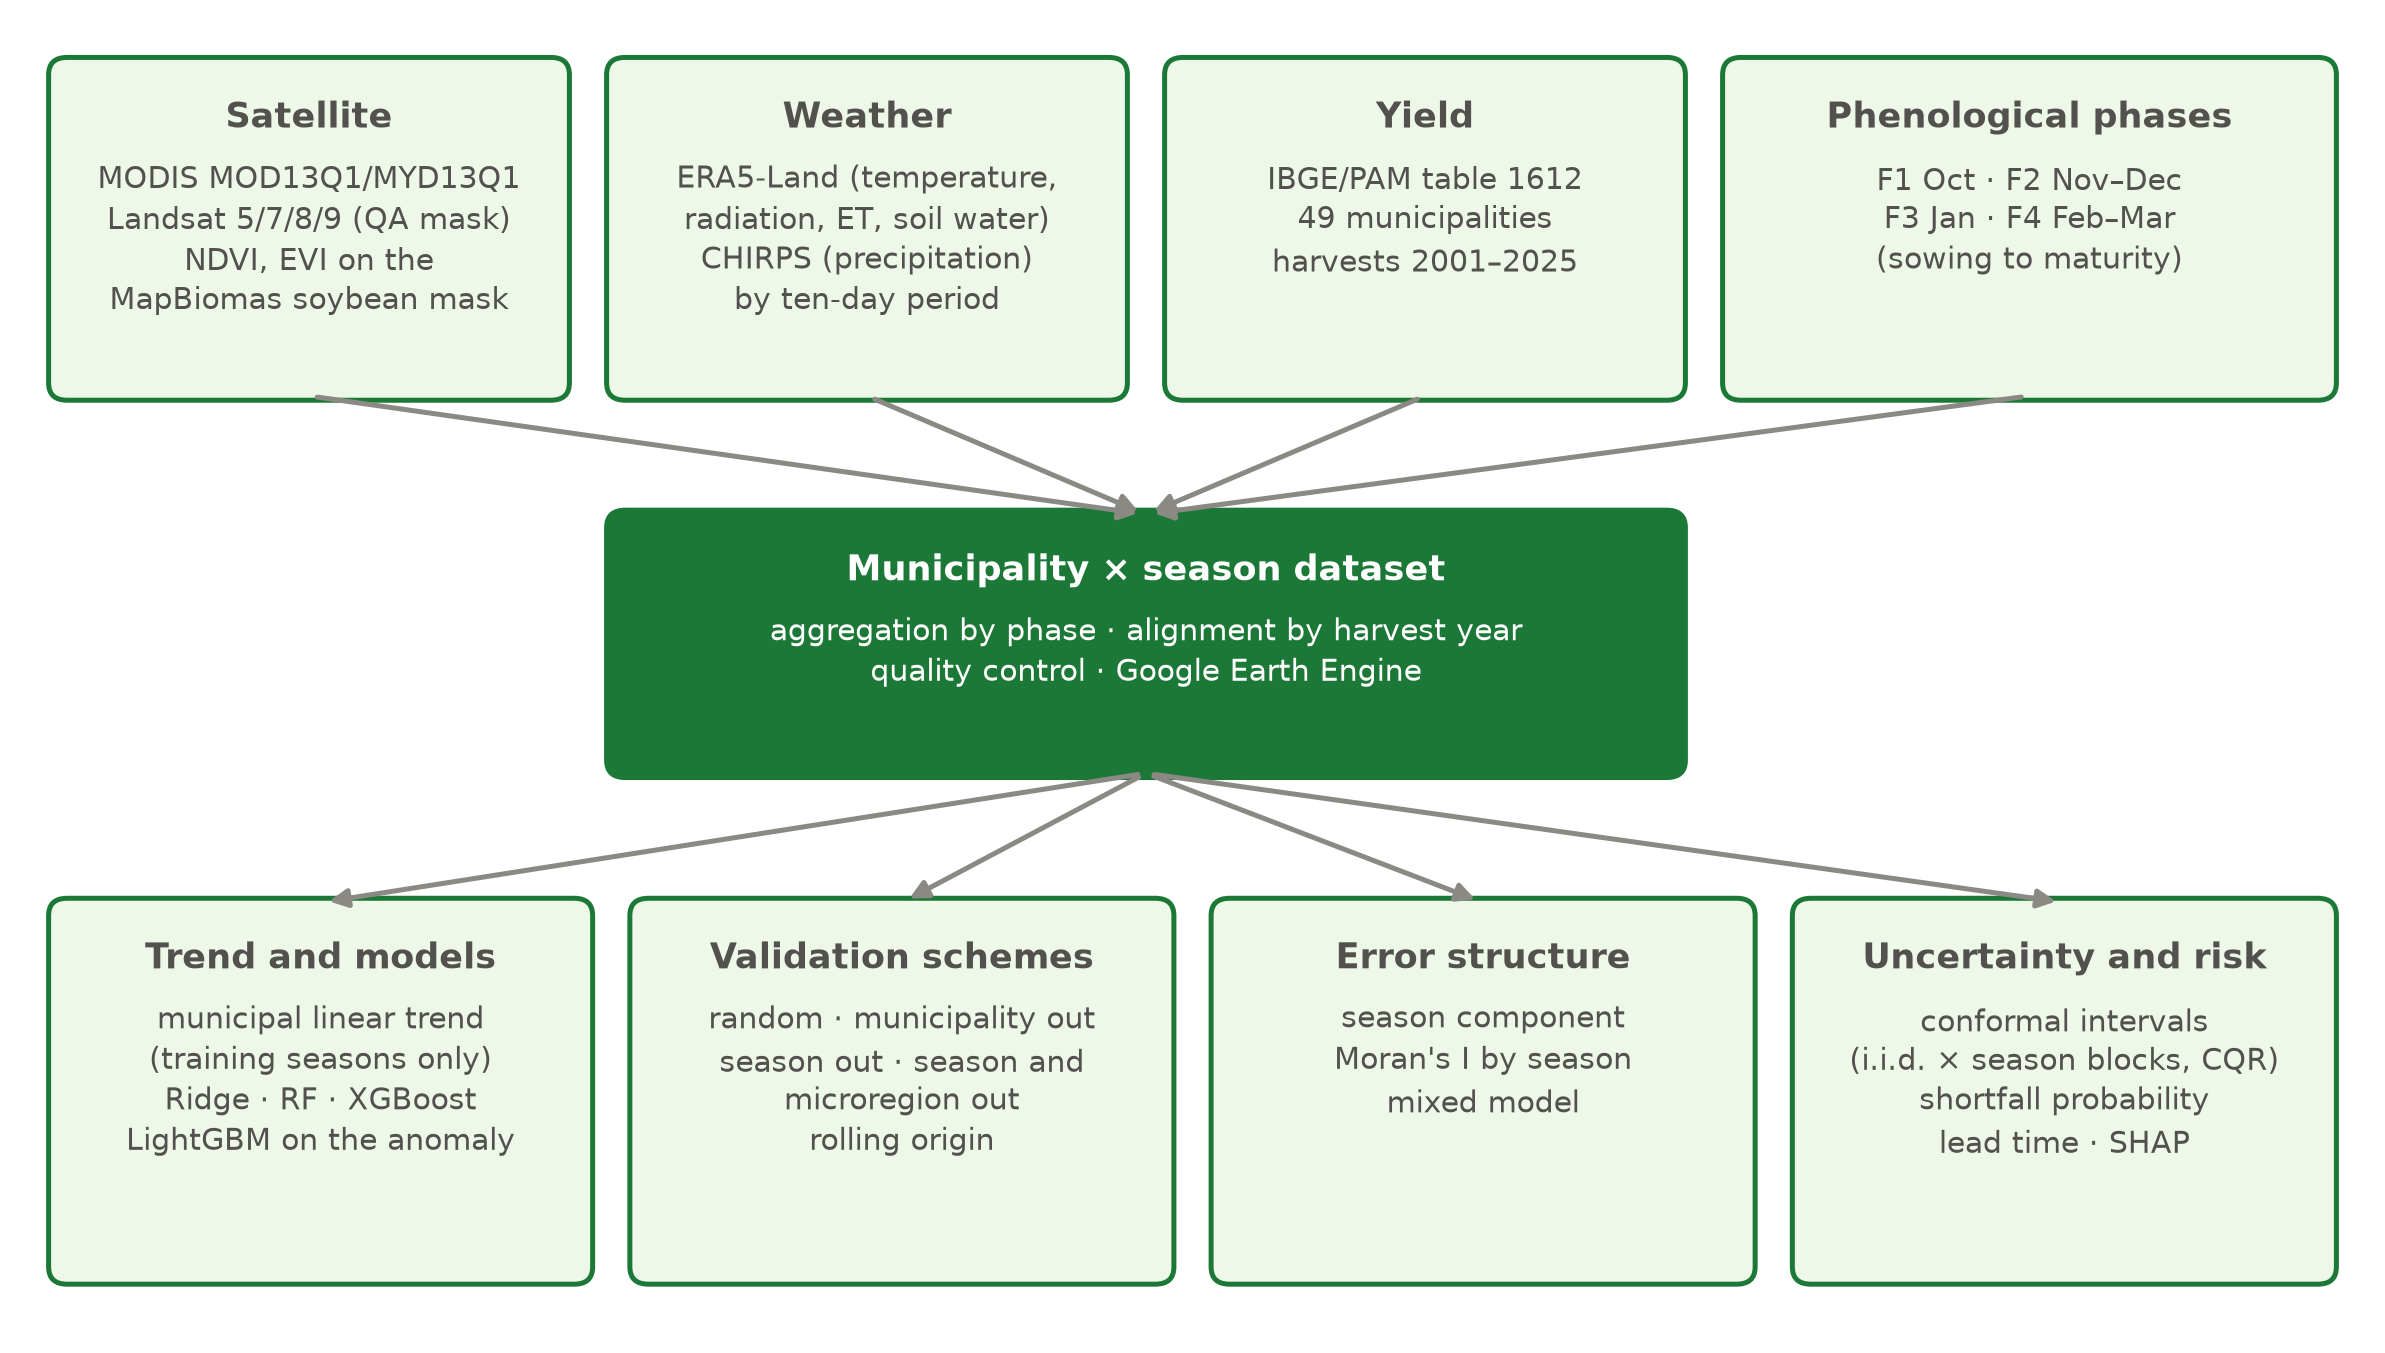
\includegraphics[width=\textwidth]{figuras/fig_fluxograma.png}
\caption{Data, dataset construction and analyses of the study.}
\label{fig:fluxo}
\end{figure}

\subsection{Study area and yield data}\label{sec:area}
The study covered 49 of the 50 municipalities of the West mesoregion of Paraná, Brazil, in the microregions of Toledo (20 municipalities), Cascavel (18) and Foz do Iguaçu (11), between 24$^\circ$S and 26$^\circ$S and 52$^\circ$W and 55$^\circ$W (Fig.~\ref{fig:area}). Terra Roxa was excluded because its Landsat records were corrupted in the original dataset of \citet{tluszcz2025}. The region has a humid subtropical climate with hot summers (Cfa) \citep{alvares2013}, with altitudes from 218 m along the Paraná River to 726 m in the Cascavel plateau, and soybean is sown from mid-September, after the sanitary break, to November and harvested from January to March \citep{brasil2025zarc}.

\begin{figure}[ht]
\centering
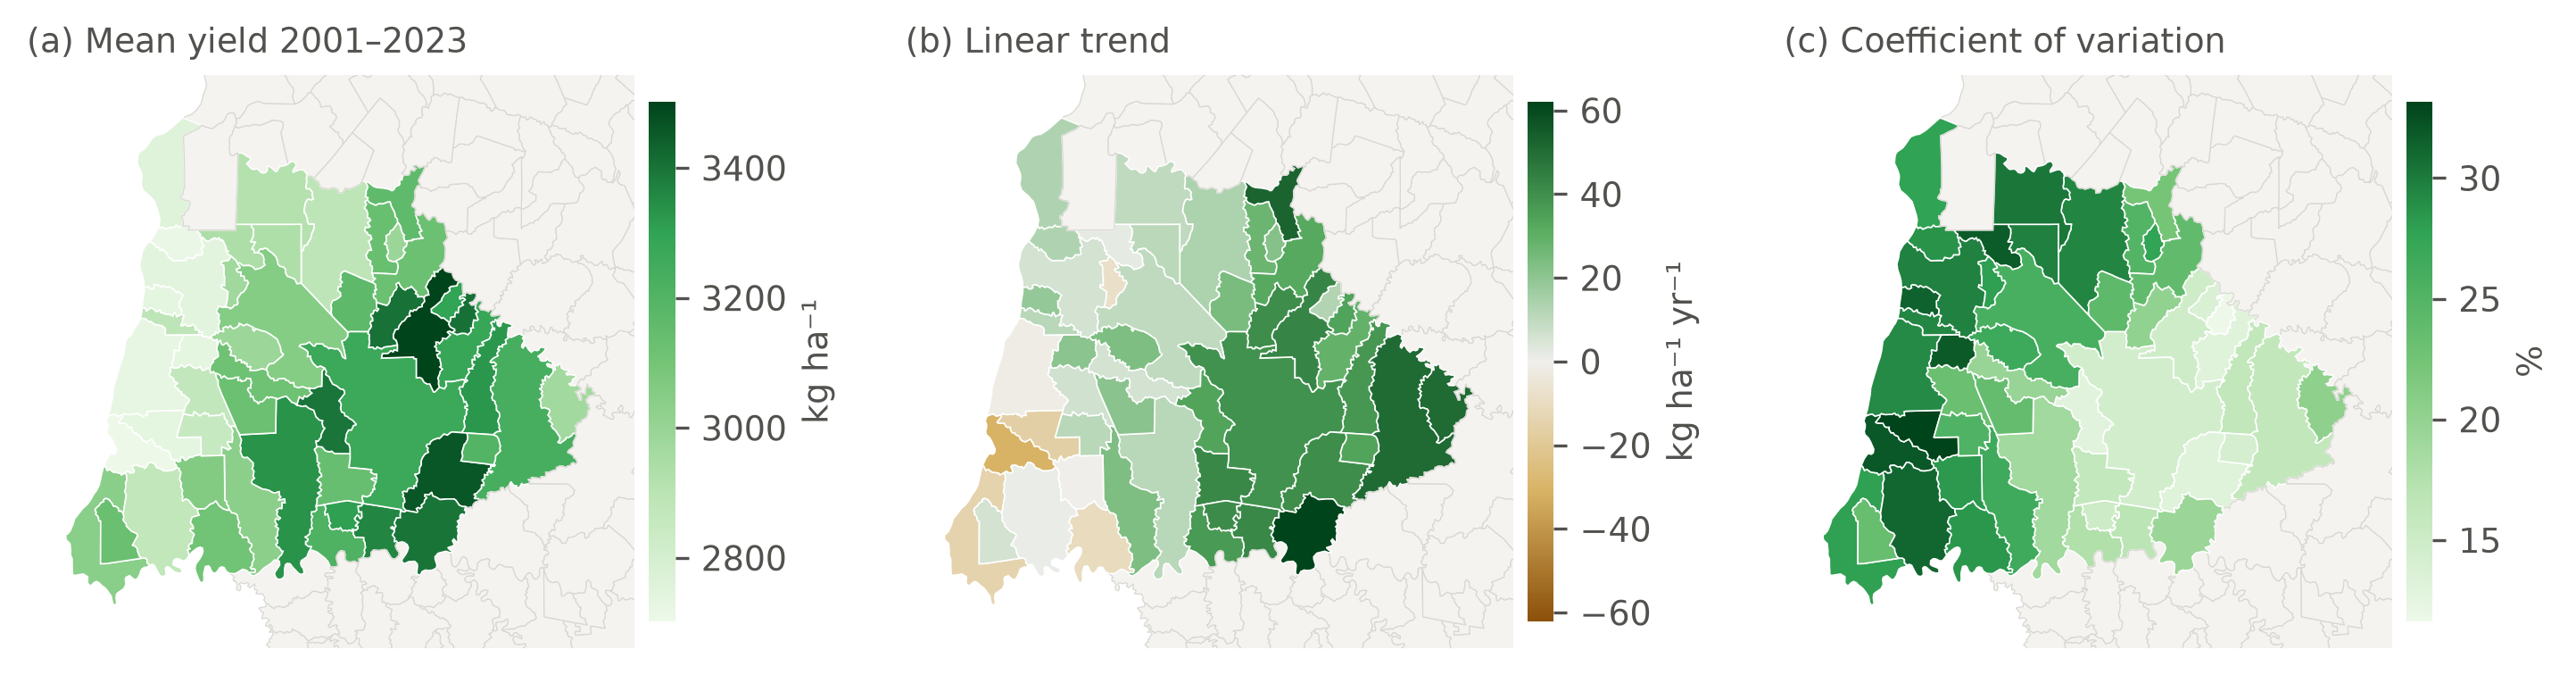
\includegraphics[width=\textwidth]{figuras/fig01_area_estudo.png}
\caption{Western Paraná: (a) mean soybean yield, (b) municipal linear trend and (c) coefficient of variation of yield, 2001--2025.}
\label{fig:area}
\end{figure}

Municipal soybean yield (kg ha$^{-1}$) for the harvests of 2001 to 2025 was obtained from the Municipal Agricultural Production survey (PAM) of the Brazilian Institute of Geography and Statistics, table 1612, variable 112 \citep{sidra}. The PAM reports the yield of each season under its harvest year; seasons are therefore identified by the harvest year $H$ (e.g.\ 2022 for the 2021/22 season), and all predictors of season $H$ were taken from 1 October of $H-1$ to 31 March of $H$. This alignment corrects the original dataset \citep{tluszcz2025}, in which the predictors of each season had been paired with the yield of the previous harvest (Section~\ref{sec:res_cv}). The final dataset had 49 municipalities $\times$ 25 seasons = 1225 records.

\subsection{Phenological phases and weather predictors}\label{sec:clima}
The season was divided into 18 calendar dekads (days 1--10, 11--20 and 21 to the end of each month) from October to March, grouped into four phases that approximately follow the development of soybean in the region \citep{fehr1977soybean,brasil2025zarc}: F1, October (sowing and emergence, dekads 1--3); F2, November and December (vegetative growth and flowering, dekads 4--9); F3, January (pod setting and beginning of seed filling, dekads 10--12); and F4, February and March (seed filling and maturation, dekads 13--18).

Daily weather was obtained from ERA5-Land \citep{munozsabater2021} and daily precipitation from CHIRPS \citep{funk2015}, averaged over each municipal polygon. For each phase, the following variables were computed: precipitation ($P$, mm), number of days with $P < 1$ mm, potential evapotranspiration ($ET_p$, mm) and actual evapotranspiration (mm), the climatic water balance,
\begin{equation}
BH_f = \sum_{k \in f} \left( P_k - ET_{p,k} \right) \label{eq:bh}
\end{equation}
where $BH_f$ is the water balance of phase $f$ (mm) and $P_k$ and $ET_{p,k}$ are the precipitation and potential evapotranspiration of dekad $k$ (mm); the mean daily mean, maximum and minimum air temperature ($^\circ$C), the absolute maximum temperature ($^\circ$C) and the number of days with maximum temperature above 32\,$^\circ$C; the mean dew-point and soil (0--7 cm) temperatures ($^\circ$C); the mean volumetric soil water content at 0--7 and 7--28 cm (m$^3$ m$^{-3}$); the accumulated global and net solar radiation (MJ m$^{-2}$); and the mean leaf area index of low vegetation.

\subsection{Vegetation indices}\label{sec:veg}
The soybean area of each municipality and season was taken from the class 39 (soybean) of the MapBiomas Collection 10 land use map of the harvest year \citep{souza2020}. NDVI and EVI were obtained from the 16-day MODIS composites of Terra (MOD13Q1) and Aqua (MYD13Q1), collection 6.1, at 250 m \citep{didan2021mod,didan2021myd}, keeping only pixels with good or marginal quality (SummaryQA $\le$ 1) and with at least 50\% of their area mapped as soybean. Landsat 5 TM, 7 ETM+, 8 OLI and 9 OLI-2 Collection 2 surface reflectance images were also processed at 30 m, after masking clouds, cloud shadows, cirrus and snow with the QA\_PIXEL band \citep{foga2017}, with
\begin{equation}
\mathrm{NDVI} = \frac{\rho_{NIR} - \rho_{R}}{\rho_{NIR} + \rho_{R}} \label{eq:ndvi}
\end{equation}
\begin{equation}
\mathrm{EVI} = 2.5\,\frac{\rho_{NIR} - \rho_{R}}{\rho_{NIR} + 6\,\rho_{R} - 7.5\,\rho_{B} + 1} \label{eq:evi}
\end{equation}
where $\rho_{NIR}$, $\rho_{R}$ and $\rho_{B}$ are the surface reflectances in the near-infrared, red and blue bands, obtained from the digital numbers as $\rho = 2.75\times10^{-5}\,DN - 0.2$.

For each image, NDVI and EVI were averaged over the soybean pixels of each municipality, and the observation was kept only when valid pixels covered at least 30\% of the soybean area and the index was within $[0, 1]$. Observations were assigned to dekads by date, and the maximum and mean of each index were computed by phase, together with the seasonal maximum. To evaluate whether Landsat adds information to MODIS, a second dataset was built in which Landsat dekad values were converted to the MODIS scale by the linear regression fitted on the dekads observed by both sensors (NDVI$_{MODIS}$ = 0.191 + 0.788 NDVI$_{Landsat}$ and EVI$_{MODIS}$ = 0.110 + 0.812 EVI$_{Landsat}$, $r = 0.96$, $n$ = 13{,}081 dekads) and averaged with MODIS; the two datasets were compared under the main validation scheme.

The final set had 93 predictors (Supplementary Table~S1), including clay and sand content \citep{tluszcz2025}, latitude, longitude, altitude and the soybean area of each municipality and season.

\subsection{Technological trend and yield anomaly}\label{sec:trend}
Yield was decomposed into a technological trend and an anomaly,
\begin{equation}
y_{it} = a_i + b_i\,(t - 2010) + \varepsilon_{it} \label{eq:trend}
\end{equation}
where $y_{it}$ is the yield of municipality $i$ in season $t$ (kg ha$^{-1}$), $a_i$ and $b_i$ are the intercept (kg ha$^{-1}$) and the slope (kg ha$^{-1}$ year$^{-1}$) of the municipal trend, fitted by least squares on the training seasons only, and $\varepsilon_{it}$ is the yield anomaly (kg ha$^{-1}$). The models predicted $\varepsilon_{it}$ from the predictors, and the yield forecast was the trend plus the predicted anomaly, $\hat{y}_{it} = \hat{a}_i + \hat{b}_i\,(t-2010) + \hat{\varepsilon}_{it}$. The trend alone was used as the reference forecast. Quadratic municipal trends and a regional trend (common slope with municipal intercepts) were tested as alternatives \citep{lobell2010,Schwalbert2020}.

\subsection{Machine-learning models}\label{sec:models}
Four regression models were compared: ridge regression, random forest \citep{breiman2001}, XGBoost \citep{chen2016} and LightGBM \citep{ke2017}. Missing predictors were imputed with the training mean for ridge regression and random forest and handled natively by the boosting models. Hyperparameters were selected inside each training set by grid search with five-fold cross-validation grouped by season, so that no season of the test set, nor any season of the inner validation folds, was used to train the model being evaluated (nested cross-validation). The grids were the regularisation strength of ridge regression ($10^{-1}$ to $10^{4}$), the minimum leaf size (1, 5, 15) and the fraction of predictors per split (0.33, 1) of random forest, the maximum depth (2, 3, 5) and learning rate (0.01, 0.03) of XGBoost, and the number of leaves (7, 15, 31), learning rate (0.01, 0.03) and minimum leaf size (10, 30) of LightGBM.

\subsection{Validation schemes}\label{sec:cv}
Four validation schemes were compared (Fig.~\ref{fig:esquemas}): (i) a random 70/30 split, repeated with 20 seeds, with the trend fitted on all seasons, as in the original study \citep{tluszcz2025} and in several yield-forecasting studies \citep{Torsoni2023,BarbosadosSantos2021}; (ii) leave-one-municipality-out, with the regional mean of the training municipalities in each season as the trend; (iii) leave-one-season-out (LOSO), in which all municipalities of the test season were withheld and the trend was refitted without it; and (iv) a rolling origin, in which each season from 2008 onwards was forecast with models trained only on previous seasons \citep{tashman2000}. Scheme (iii) was adopted as the main scheme because it reproduces the operational situation of forecasting a new season from past seasons while using all seasons for evaluation; a combined season and microregion scheme was not necessary, because no observation of the test season enters the training set in LOSO \citep{roberts2017}. To show what schemes (i) and (iii) measure, they were also applied to the original dataset, with and without the one-year misalignment of yields, and to a replica of its feature engineering by calendar year.

\begin{figure}[ht]
\centering
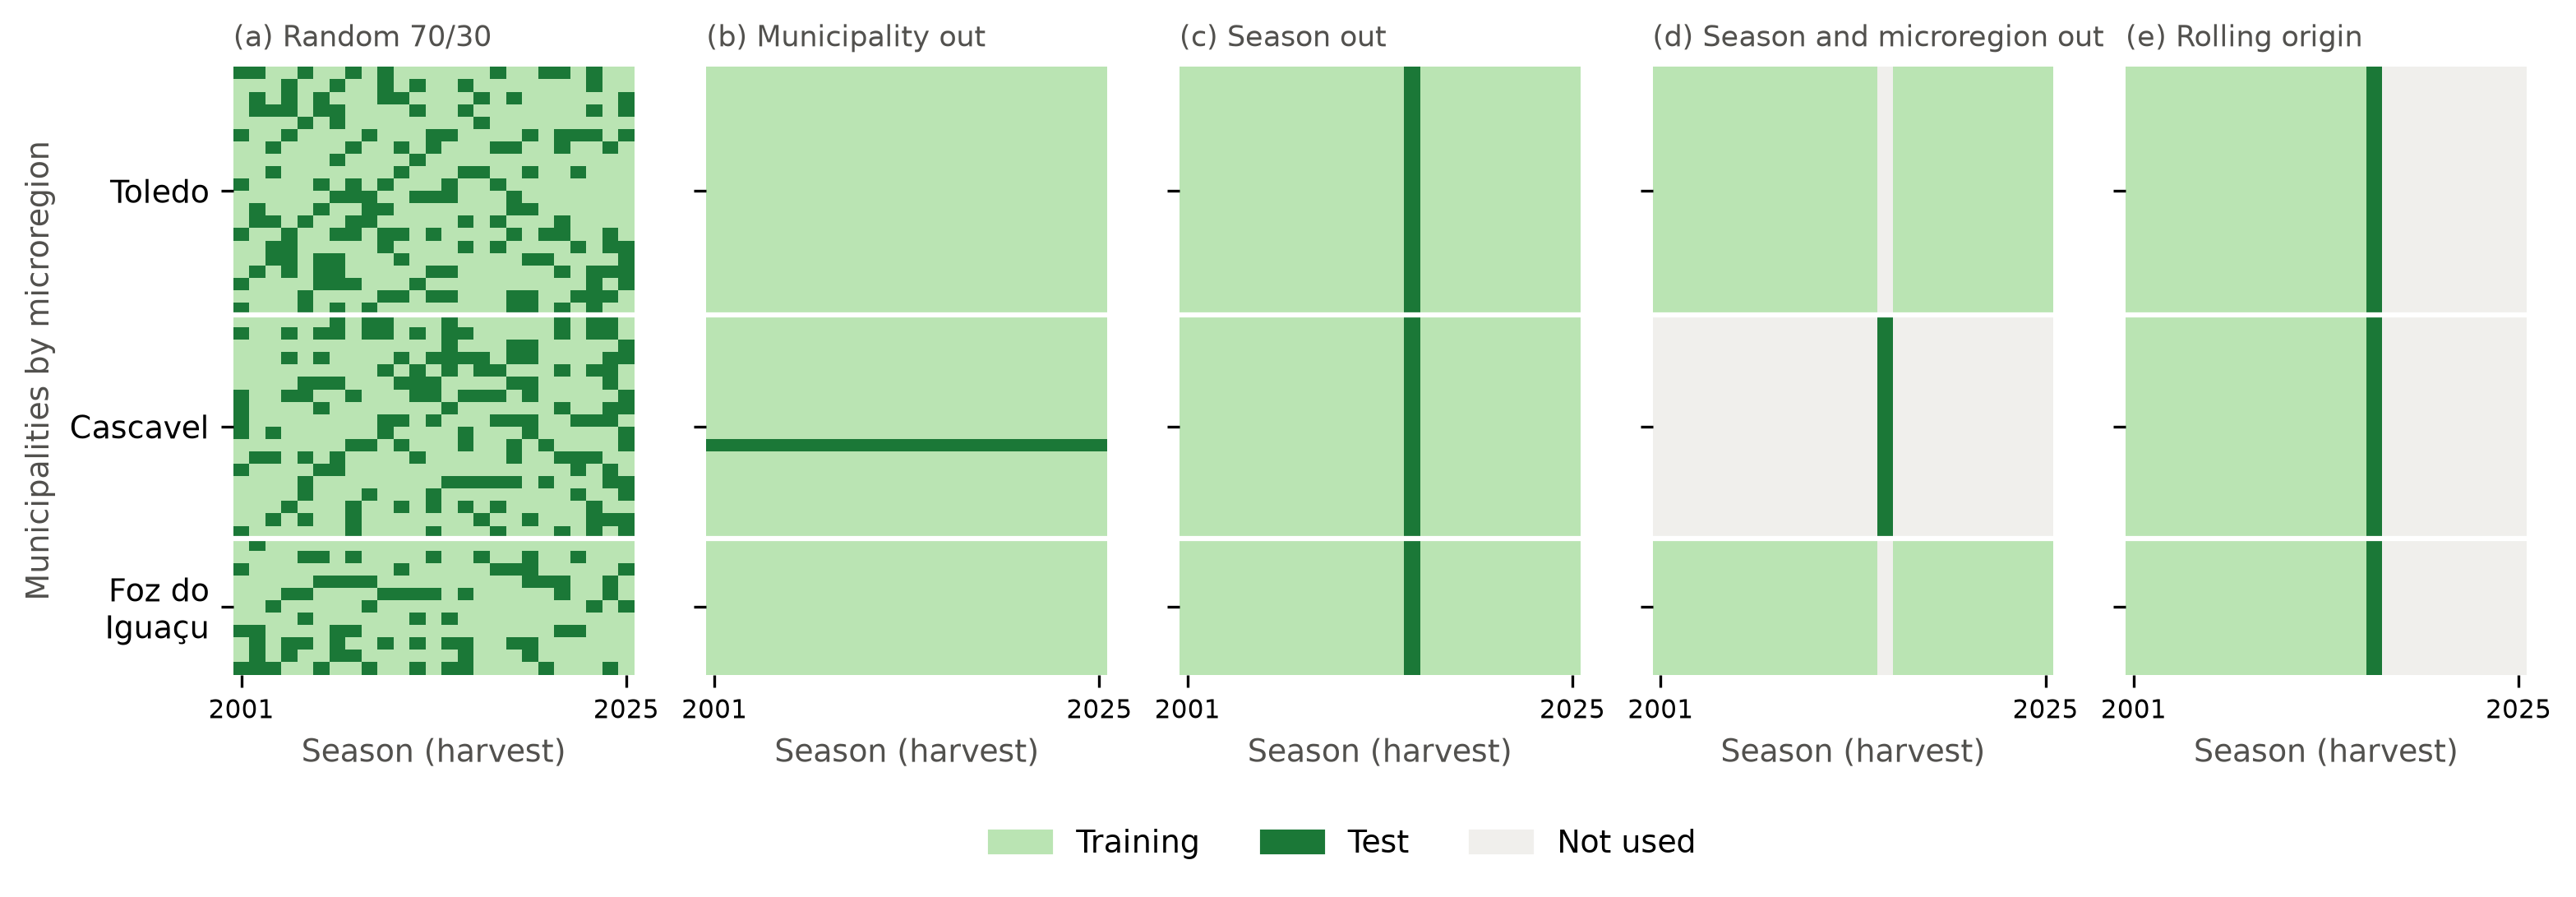
\includegraphics[width=\textwidth]{figuras/fig_esquemas_validacao.png}
\caption{Training and test sets of the validation schemes for one fold, shown as a matrix of municipalities (rows, by microregion) and seasons (columns).}
\label{fig:esquemas}
\end{figure}

Performance was assessed with the coefficient of determination ($R^2$), the mean absolute error (MAE), the root mean square error (RMSE), which together describe the average and the large errors \citep{chai2014}, and the skill over the trend,
\begin{equation}
S = 1 - \frac{\sum_{i,t} \left( y_{it} - \hat{y}_{it} \right)^2}{\sum_{i,t} \left( y_{it} - \hat{y}^{\,\mathrm{trend}}_{it} \right)^2} \label{eq:skill}
\end{equation}
where $\hat{y}_{it}$ is the forecast of the model and $\hat{y}^{\,\mathrm{trend}}_{it}$ that of the trend alone (kg ha$^{-1}$); $S > 0$ indicates that the model improves on the trend. Differences in mean squared error between models were tested with a bootstrap of whole seasons (2000 replicates), which preserves the dependence among municipalities of the same season \citep{diebold1995}.

\subsection{Spatio-temporal structure of the errors}\label{sec:errors}
The LOSO residuals $r_{it} = y_{it} - \hat{y}_{it}$, and the observed anomalies, were decomposed with a linear mixed model with crossed random effects of season and municipality,
\begin{equation}
r_{it} = \mu + u_t + v_i + e_{it}, \quad u_t \sim N(0, \sigma^2_u),\; v_i \sim N(0, \sigma^2_v),\; e_{it} \sim N(0, \sigma^2_e) \label{eq:misto}
\end{equation}
where $\mu$ is the mean residual, $u_t$ the effect of season $t$, common to all municipalities, $v_i$ the effect of municipality $i$ and $e_{it}$ the remaining error, with variances $\sigma^2_u$, $\sigma^2_v$ and $\sigma^2_e$ (kg$^2$ ha$^{-2}$) estimated by restricted maximum likelihood. The spatial dependence of the residuals within each season was evaluated with Moran's $I$ \citep{moran1950},
\begin{equation}
I_t = \frac{\sum_i \sum_j w_{ij}\, z_{it} z_{jt}}{\sum_i z_{it}^2} \label{eq:moran}
\end{equation}
where $z_{it}$ is the residual of municipality $i$ in season $t$ minus the mean of the season and $w_{ij}$ are row-standardised weights equal to 1/6 for the six nearest municipal centroids and 0 otherwise; significance was assessed with 999 permutations. The range of the dependence was estimated by fitting an exponential model, $\gamma(h) = c_0 + c\,[1 - \exp(-h/a)]$, to the empirical semivariogram of the within-season residuals, where $h$ is the distance between centroids (km), $c_0$ the nugget, $c_0 + c$ the sill and $3a$ the practical range (km).

\subsection{Prediction intervals}\label{sec:conformal}
Prediction intervals with a nominal coverage of 90\% were obtained by three methods, always calibrated on seasons other than the test season: (i) split conformal intervals with half-width equal to the 0.9 quantile of the absolute LOSO residuals of the other seasons, which assume exchangeable municipal errors \citep{lei2018}; (ii) Gaussian intervals with variance $\sigma^2_u + \sigma^2_v + \sigma^2_e$ from Eq.~\ref{eq:misto} fitted without the test season; and (iii) conformalised quantile regression (CQR) \citep{romano2019}, with the 0.05 and 0.95 quantiles of the anomaly predicted by LightGBM and corrected by the conformity scores of the other seasons. For the regional mean yield, the naive interval assumed independent municipal errors (half-width $q_{0.9}/\sqrt{n_t}$, where $n_t$ is the number of municipalities), the mixed model used the variance $\sigma^2_u + (\sigma^2_v + \sigma^2_e)/n_t$, and a season-block conformal interval used the 0.9 quantile of the absolute regional mean residuals of the other seasons. Exchangeability, which underlies conformal guarantees, does not hold among municipalities of the same season \citep{barber2023,mao2024}; the comparison therefore measures the cost of ignoring this dependence.

\subsection{Shortfall risk}\label{sec:risk}
A shortfall was defined as a yield below 70, 80 or 90\% of the trend. Its probability was estimated as the fraction of the LOSO residuals of the other seasons that, added to the forecast, produced a yield below the threshold, and was compared with the climatological frequency of shortfall in the other seasons by the Brier score \citep{brier1950},
\begin{equation}
BS = \frac{1}{N}\sum_{i,t} \left( p_{it} - o_{it} \right)^2, \qquad BSS = 1 - \frac{BS}{BS_{clim}} \label{eq:brier}
\end{equation}
where $p_{it}$ is the forecast probability, $o_{it}$ equals 1 if a shortfall occurred and 0 otherwise, $N$ is the number of forecasts and $BS_{clim}$ is the Brier score of the climatological frequency \citep{gneiting2007}. The area under the ROC curve (AUC) and reliability diagrams complemented the evaluation.

\subsection{Lead time and predictor contributions}\label{sec:lead}
LOSO was repeated with the predictors of phases F1, F1--F2, F1--F3 and F1--F4, which correspond to forecasts issued at the end of October, at the end of December, at the beginning of February and at harvest. To test whether the El Niño--Southern Oscillation provides an earlier signal, the Oceanic Niño Index of August--October of the sowing year \citep{noaa_oni}, available at the end of October, was correlated with the regional yield anomaly and added to the predictors of phase F1 and of the whole season. The contribution of the predictors was summarised by the mean absolute SHAP value \citep{lundberg2017} of the final model, aggregated by phase and by variable.

%%

%% ---------------------------------------------------------------
\section{Results and discussion}\label{sec:rd}

\subsection{Yield variability in western Paraná}\label{sec:res_area}
Between 2001 and 2025, the mean municipal soybean yield ranged from 2702 to 3502 kg ha$^{-1}$ and the coefficient of variation between seasons from 11.6 to 33.2\% (Fig.~\ref{fig:area}). Yields were higher and more stable in the east, in the Cascavel microregion (mean of 3295 kg ha$^{-1}$ and coefficient of variation of 16\%), than in the west, along the Paraná River, in the Toledo and Foz do Iguaçu microregions (2923 and 3001 kg ha$^{-1}$, 28 and 27\%); the coefficient of variation decreased from west to east ($r = -0.75$ with longitude). The municipal trends had a median of 20.7 kg ha$^{-1}$ year$^{-1}$, from $-30.9$ to 62.1 kg ha$^{-1}$ year$^{-1}$, a gain attributed to the continuous release of adapted cultivars and to improvements in crop management \citep{Cattelan2018,gazzoni2018saga}; six municipalities of the south-west had negative trends, which reflects the concentration of severe losses in the last seasons of the series in that area rather than a loss of technology. Because the trend is fitted on few seasons, a single extreme season near the end of the series changes its slope, which is one reason why it must be refitted in each fold. The regional mean yield was more than 15\% below the trend in six seasons, with losses of 19\% in 2004, 25\% in 2006, 28\% in 2009, 38\% in 2012, 17\% in 2019 and 53\% in 2022, and in five of them (2004, 2006, 2009, 2012 and 2022) the shortfall below 80\% of the trend affected more than half of the municipalities. These losses coincided with dry spells in November--January, as in the 2021/22 season, when the water balance of phase F2 reached $-928$ mm against a median of $-342$ mm in the other seasons, and the maximum EVI of January fell to 0.40 against 0.74 \citep{idrparana2022}. The year-to-year variation of soybean yield in the region is therefore dominated by events that affect most municipalities at the same time, the condition in which the dependence between observations is strongest.

\subsection{What each validation scheme measures}\label{sec:res_cv}
The random 70/30 split produced $R^2$ between 0.79 and 0.83 for all models and datasets (Table~\ref{tab:cv}; Fig.~\ref{fig:cv}), including the replica of the earlier study (0.80) and the original dataset in which the predictors of each season had been paired with the yield of the previous harvest (0.81). In that misaligned dataset, the correlation between the maximum NDVI of January and the yield anomaly of the same row was $-0.06$, and leaving out whole seasons gave an $R^2$ of $-0.39$, a forecast worse than the trend alone. After correcting the alignment, the same model and predictors reached $R^2 = 0.25$ under LOSO, and with the new dataset, extracted with quality and cloud masks, the $R^2$ reached 0.47 for LightGBM and 0.59 for ridge regression. The leave-one-municipality-out scheme gave $R^2 = 0.79$ for LightGBM, but the trend computed from the other municipalities in the same season already gave 0.60, so that most of its skill came from the yields of neighbouring municipalities in the test season.

\begin{table}[ht]
\caption{Test performance by dataset, validation scheme and model. Skill: Eq.~\ref{eq:skill}; random split: mean of 20 seeds (standard deviation of $R^2 \le 0.03$).}
\label{tab:cv}
\begin{tabular}{@{}lllrrr@{}}
\toprule
Dataset & Scheme & Model & $R^2$ & MAE (kg ha$^{-1}$) & Skill \\
\midrule
Earlier study (replica) & Random & LightGBM & 0.80 & 236 & 0.77 \\
Earlier data, misaligned & Random & LightGBM & 0.81 & 237 & 0.77 \\
Earlier data, misaligned & LOSO & LightGBM & $-0.39$ & 622 & $-0.35$ \\
Earlier data, aligned & LOSO & LightGBM & 0.25 & 477 & 0.27 \\
New data & Random & LightGBM & 0.83 & 216 & 0.80 \\
New data & Municipality out & LightGBM & 0.79 & 245 & 0.48 \\
New data & LOSO & Trend & 0.02 & 547 & 0 \\
New data & LOSO & Ridge & \textbf{0.59} & \textbf{361} & \textbf{0.58} \\
New data & LOSO & Random forest & 0.45 & 411 & 0.44 \\
New data & LOSO & XGBoost & 0.47 & 403 & 0.46 \\
New data & LOSO & LightGBM & 0.47 & 404 & 0.46 \\
New data & Rolling origin & Trend & $-0.20$ & 665 & 0 \\
New data & Rolling origin & Ridge & 0.37 & 500 & 0.48 \\
New data & Rolling origin & LightGBM & 0.28 & 524 & 0.40 \\
\botrule
\end{tabular}
\end{table}

\begin{figure}[ht]
\centering
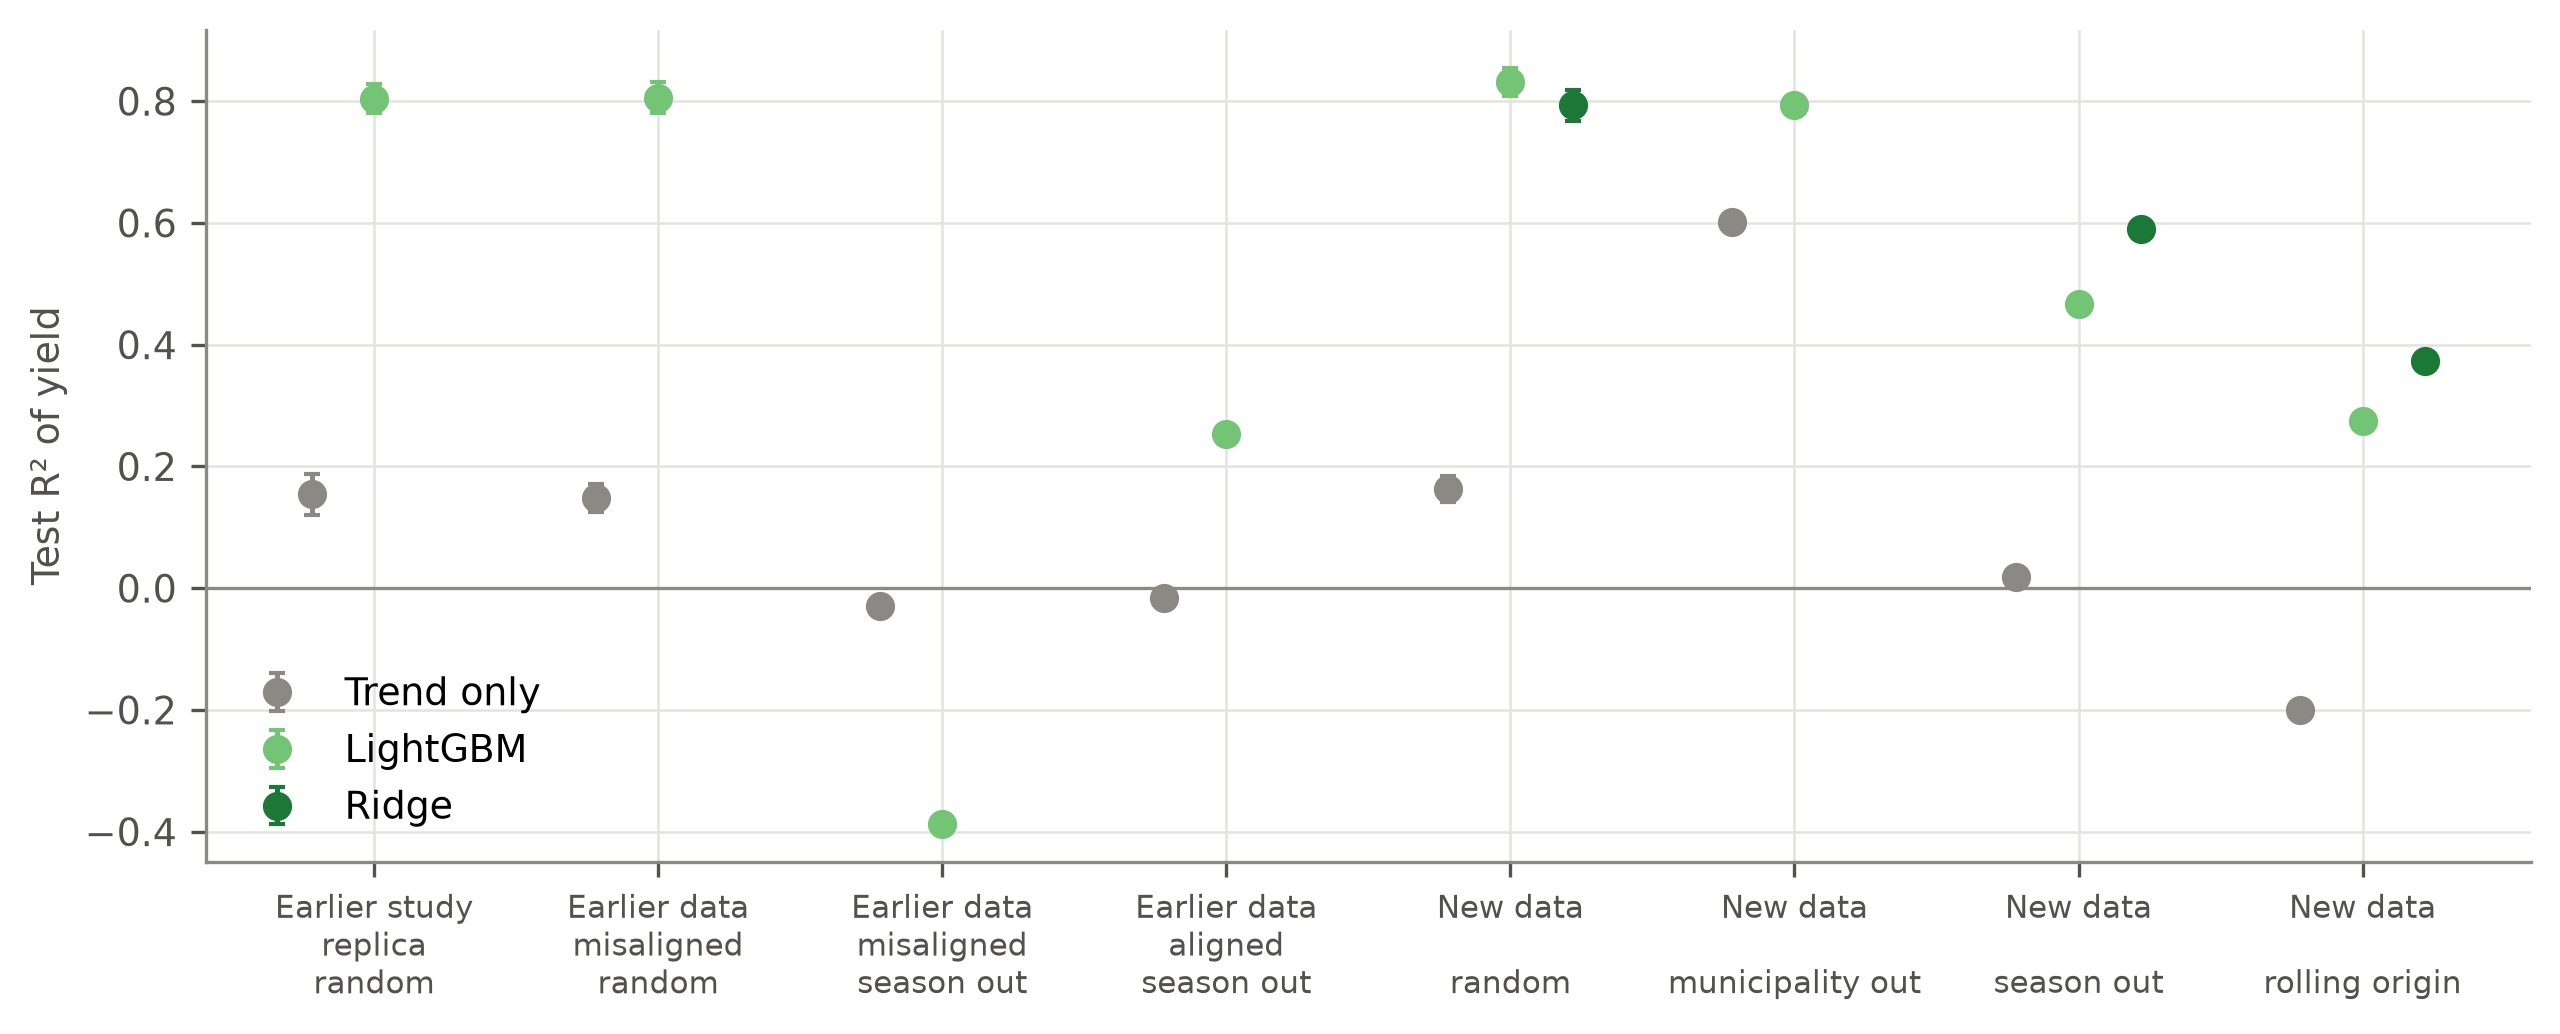
\includegraphics[width=\textwidth]{figuras/fig02_validacoes.png}
\caption{Test $R^2$ of the trend alone, LightGBM and ridge regression under each dataset and validation scheme. Error bars: standard deviation over 20 random splits.}
\label{fig:cv}
\end{figure}

The random split therefore reported the same skill with the correct and with the wrong pairing of predictors and yields. Because each season contributes 49 records with nearly the same weather, a random split places about 70\% of the municipalities of every season in the training set, and the model only has to recognise the season from its weather and assign the anomaly of the neighbouring municipalities; this requires no relationship between the predictors and the yield response, as shown by the misaligned dataset. This is the form of dependence-induced optimism described for ecological and remote-sensing models by \citet{roberts2017} and \citet{ploton2020}, and it explains the high $R^2$ reported in the earlier study \citep{tluszcz2025}. Studies that forecast soybean yield with random or location-based splits \citep{Torsoni2023,BarbosadosSantos2021} should therefore be interpreted as estimates of the spatial interpolation of yields within a season, not of the forecast of a new season. The difference between LOSO and the rolling origin (0.58 and 0.48 of skill for ridge regression) is the cost of training with fewer seasons in the first years of the rolling scheme, and both schemes confirmed that the predictors carry information that the trend does not have.

\subsection{Model, trend and sensor choices}\label{sec:res_mod}
Under LOSO, ridge regression reduced the mean squared error of the trend by 58\%, against 44 to 46\% for the tree-based models (Table~\ref{tab:cv}). The bootstrap of seasons confirmed the gain of ridge regression over the trend (difference in MSE of $-3.15\times10^{5}$ kg$^2$ ha$^{-2}$, 95\% interval from $-6.59\times10^{5}$ to $-0.95\times10^{5}$), whereas its advantage over random forest, XGBoost and LightGBM, about $-0.7\times10^{5}$ kg$^2$ ha$^{-2}$, had 95\% intervals that included zero (upper limits from $0.09\times10^{5}$ to $0.13\times10^{5}$), with 4 to 5\% of the bootstrap replicates favouring the tree models (Supplementary Table~S3). The selected regularisation of ridge regression was strong (median $\alpha = 316$, from 100 to 1000 over the 25 LOSO folds), and the quadratic and regional trends changed the skill by less than 0.02 (0.577 and 0.596, against 0.583 for the linear municipal trend). Adding Landsat to MODIS did not improve LightGBM (skill of 0.464 against 0.457; difference in MSE with a 95\% interval from $-1.7\times10^{4}$ to $0.9\times10^{4}$ kg$^2$ ha$^{-2}$), although the two sensors were highly correlated after calibration (NDVI$_{MODIS}$ = 0.191 + 0.788 NDVI$_{Landsat}$, $r = 0.96$, $n$ = 13{,}081 dekads).

The advantage of a strongly regularised linear model reflects the effective sample size of the problem. Although the dataset has 1225 records, the information about the response of yield to weather comes from 25 seasons, most of which are similar, and from five seasons with widespread losses. With 73\% of the variance of the anomalies shared by all municipalities of a season (Section~\ref{sec:res_err}), the design effect $1 + (n_t - 1)\rho$, where $\rho$ is the fraction of the variance due to the season, is 36, and the 1225 records are equivalent to about 34 independent observations; for the residuals of ridge regression ($\rho = 0.40$) they are equivalent to about 61. In this setting, flexible models fitted to 24 seasons tend to learn the particularities of the few extreme seasons, which do not repeat in the same way. \citet{vonBloh2023} also reported that the relative errors of municipal soybean forecasts in Brazil ranged from 4\% in the centre-north to more than 30\% in the south, where weather variability is highest, and \citet{lischeid2022} cautioned that machine-learning yield models are limited by the information contained in the data \inserir{conferir no texto completo}. The absence of gain from Landsat is consistent with the large soybean fields of western Paraná, which are well resolved by MODIS at 250 m, and with the higher temporal frequency of MODIS (Terra and Aqua), which matters more than spatial detail for municipal averages.

\subsection{Accuracy across scales and comparison with previous studies}\label{sec:res_escala}
The accuracy of the LOSO forecasts increased with aggregation: $R^2$ was 0.59 for municipalities, 0.71 for the three microregions and 0.74 for the regional mean, and the relative RMSE decreased from 15.4\% to 11.7\% and 9.6\%. Averaging removes the within-season variation among municipalities, which the predictors explained poorly ($R^2 = 0.17$, Section~\ref{sec:res_err}), and leaves the season signal, which they explained well. The municipal error is close to the mean relative RMSE of 16\% reported by \citet{vonBloh2023} for Brazilian municipalities and lower than the errors above 30\% they reported for southern Brazil, and the MAE of 361 kg ha$^{-1}$ is larger than the 240 kg ha$^{-1}$ obtained by \citet{Schwalbert2020} one month before harvest in southern Brazil; the comparison is approximate, because the periods, regions and validation designs differ, and the series analysed here includes losses of 38\% and 53\% that dominate the squared errors. The $R^2$ of 0.88 reported for soybean in the MATOPIBA region \citep{BarbosadosSantos2021} and the 0.70 of the earlier study of western Paraná \citep{tluszcz2025} were obtained with random splits and are comparable to the 0.83 obtained here under the same scheme, not to the season-blocked values.

\subsection{Spatio-temporal structure of the errors}\label{sec:res_err}
The season effect explained 73\% of the variance of the observed yield anomalies ($4.50\times10^{5}$ of $6.18\times10^{5}$ kg$^2$ ha$^{-2}$) and the municipality effect was negligible, because the municipal trend already removes the mean level of each municipality (Fig.~\ref{fig:ic8}b). Ridge regression removed 80\% of the season variance, to $0.92\times10^{5}$ kg$^2$ ha$^{-2}$, but this component still accounted for 40\% of the residual variance. Accordingly, the forecast of the regional mean anomaly was good ($r = 0.88$, $R^2 = 0.77$; regional MAE of 230 kg ha$^{-1}$, against 487 kg ha$^{-1}$ for the trend), whereas the variation of the anomaly among municipalities within a season was poorly explained ($R^2 = 0.17$). The residuals were spatially autocorrelated within seasons, with a median Moran's $I$ of 0.31 (0.00 to 0.71) and significance at 5\% in 22 of the 25 seasons, the strongest in 2004. The semivariance of the within-season residuals increased steadily from about $0.8\times10^{5}$ kg$^2$ ha$^{-2}$ at 20 km to $2.0\times10^{5}$ kg$^2$ ha$^{-2}$ at 160 km, the largest distance with enough pairs, without reaching a sill; the fitted exponential model had a nugget of 15\% of the sill and a practical range of about 770 km, an extrapolation that indicates a dependence that decreases smoothly across the whole region rather than local clusters (Supplementary Fig.~S1).

\begin{figure}[ht]
\centering
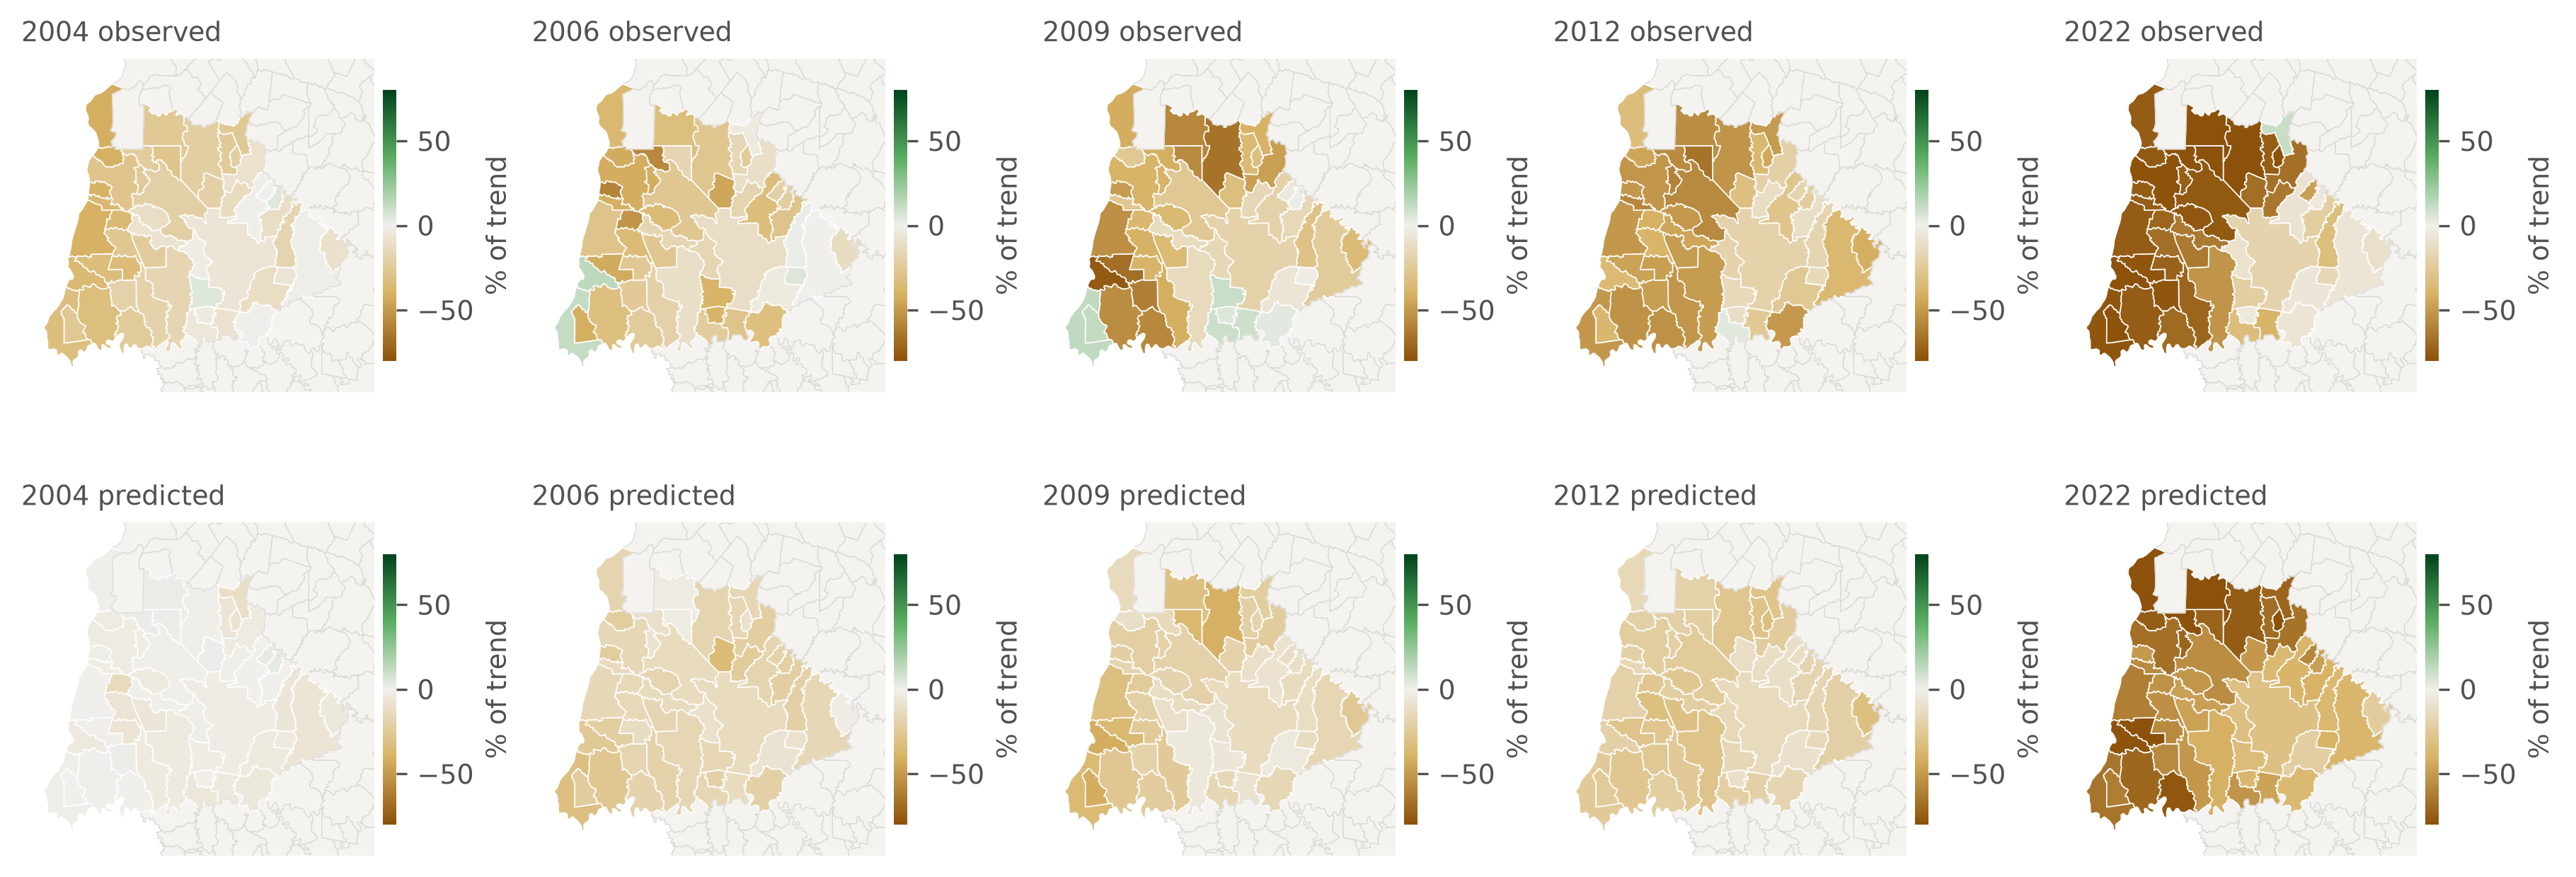
\includegraphics[width=\textwidth]{figuras/fig05_mapas_quebras.png}
\caption{Observed (top) and LOSO-predicted (bottom, ridge regression) yield anomalies, in \% of the trend, in the five seasons with shortfall below 80\% of the trend in more than half of the municipalities.}
\label{fig:quebras}
\end{figure}

The maps of the seasons with widespread losses show that the model reproduced the spatial pattern and the magnitude of the 2022 drought, with a predicted regional loss of 54\% against 53\% observed, but underestimated the losses of 2012 (21\% against 38\%), 2009 (19\% against 28\%) and 2004 (3\% against 19\%) (Fig.~\ref{fig:quebras}; Fig.~\ref{fig:ic}). In 2022 the drought began in November and reduced the maximum EVI of January to 0.40 throughout the region, against a median of 0.74 in the other seasons. In 2009 and 2012 the reduction of the index was smaller (0.55 and 0.53), and in 2004 the index was normal (0.74), although the losses were concentrated in the west; this suggests losses during seed filling, after the phase best represented by the predictors \inserir{conferir com boletins de 2004 e 2012}. Underestimation of extremes is expected from models fitted by least squares to few extreme events, particularly when the yield response to heat and drought is nonlinear \citep{schlenker2009,lobell2010}, and it is the main reason why the uncertainty of the forecasts must be quantified.

\begin{figure}[ht]
\centering
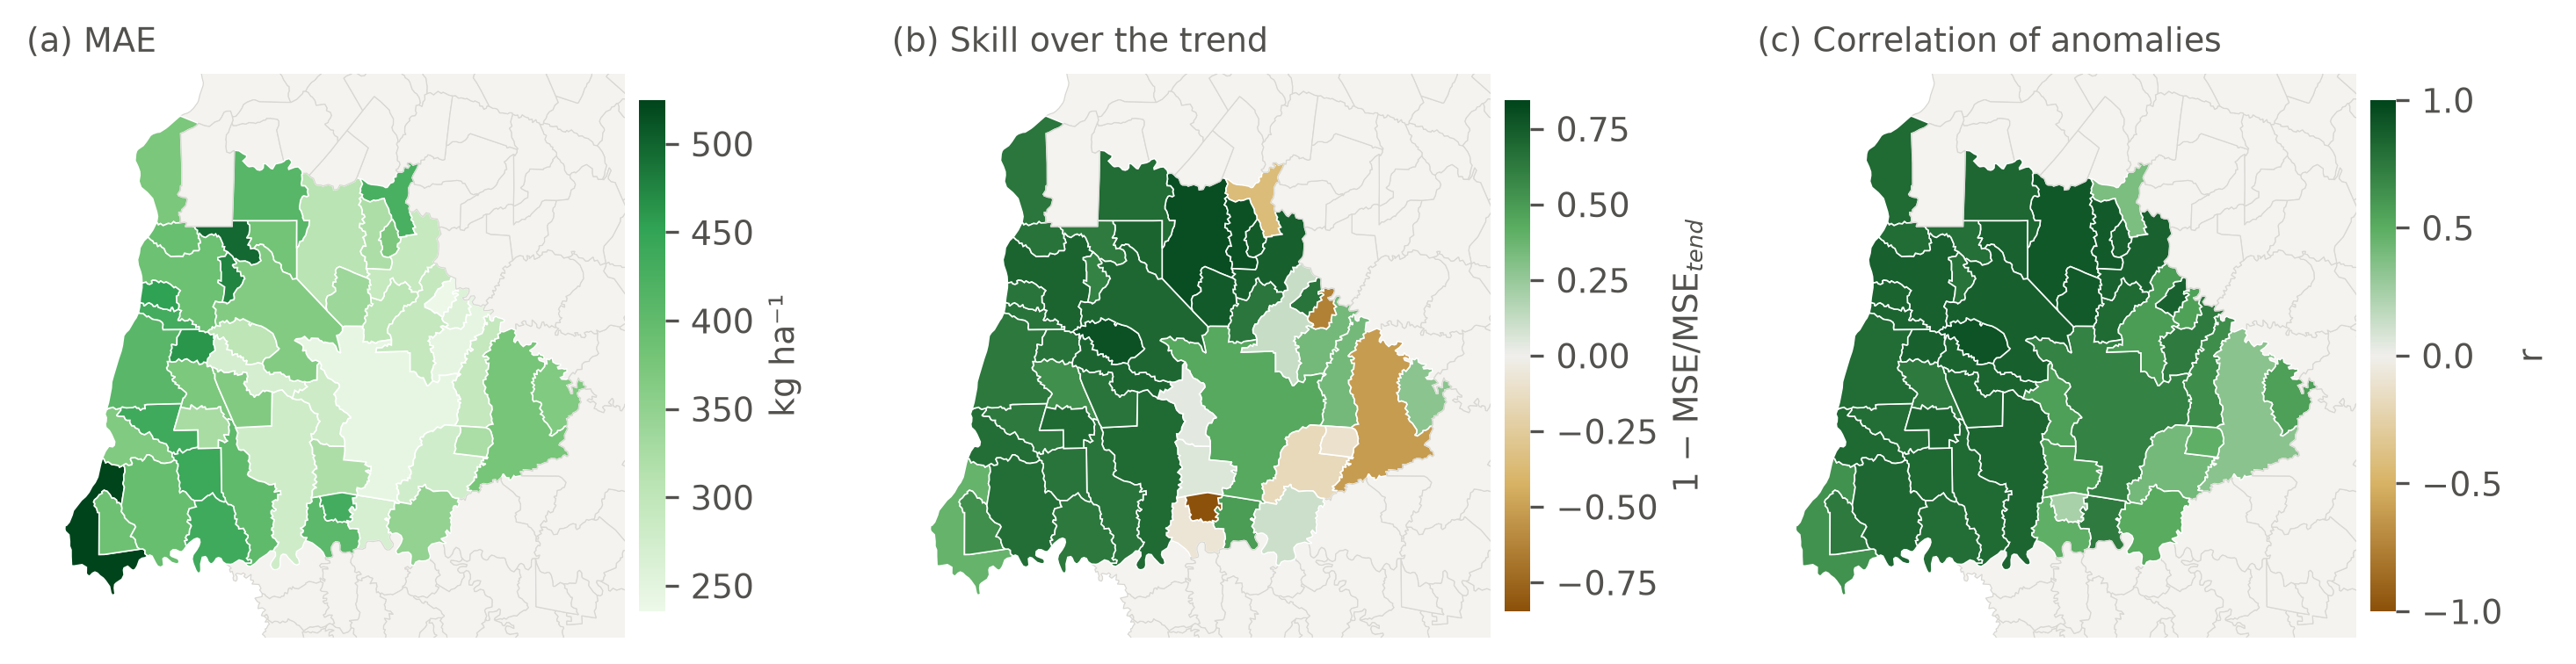
\includegraphics[width=\textwidth]{figuras/fig04_mapas_desempenho.png}
\caption{LOSO performance of ridge regression by municipality: (a) MAE, (b) skill over the trend and (c) correlation between observed and predicted anomalies.}
\label{fig:mun}
\end{figure}

By municipality, the skill over the trend had a median of 0.64 and was positive in 42 of the 49 municipalities, and the MAE ranged from 236 to 525 kg ha$^{-1}$ (Fig.~\ref{fig:mun}; Supplementary Table~S5). The skill was 0.66 in the Toledo microregion, 0.62 in Foz do Iguaçu and 0.24 in Cascavel, where six of the seven municipalities with negative skill are located (Santa Lúcia, Iguatu, Guaraniaçu, Catanduvas, Ibema and Capitão Leônidas Marques; the seventh is Formosa do Oeste). The Cascavel plateau, on the third plateau of Paraná \citep{Santos}, is higher and about 2\,$^\circ$C cooler and had the smallest losses in the drought seasons \citep{tluszcz2025,idrparana2022}, so its yield anomalies are smaller and less related to the regional weather signal that dominates the forecasts.

\subsection{Calibration of prediction intervals}\label{sec:res_ic}
At the municipal scale, the three methods reached the nominal coverage on average, with 89.4\% for split conformal intervals, 90.0\% for the mixed model and 89.5\% for CQR, and mean widths of 1547, 1581 and 1794 kg ha$^{-1}$ (Fig.~\ref{fig:ic8}a). The coverage, however, was not uniform between seasons: it fell below 80\% in six seasons for the conformal and mixed-model intervals and in five for CQR, with minima of 49\% in 2021 and 47\% (CQR) in 2022, and these were the seasons with the largest forecast errors, either losses underestimated (2004, 2009, 2012), a high yield underestimated (2020) or a yield overestimated (2021). For the regional mean yield, the naive interval, which assumes independent municipal errors, had a mean width of 221 kg ha$^{-1}$ and covered the observed mean in only 32\% of the seasons, whereas the season-block conformal and the mixed-model intervals, with widths of 999 and 1007 kg ha$^{-1}$, covered 84\% (Fig.~\ref{fig:ic}).

\begin{figure}[ht]
\centering
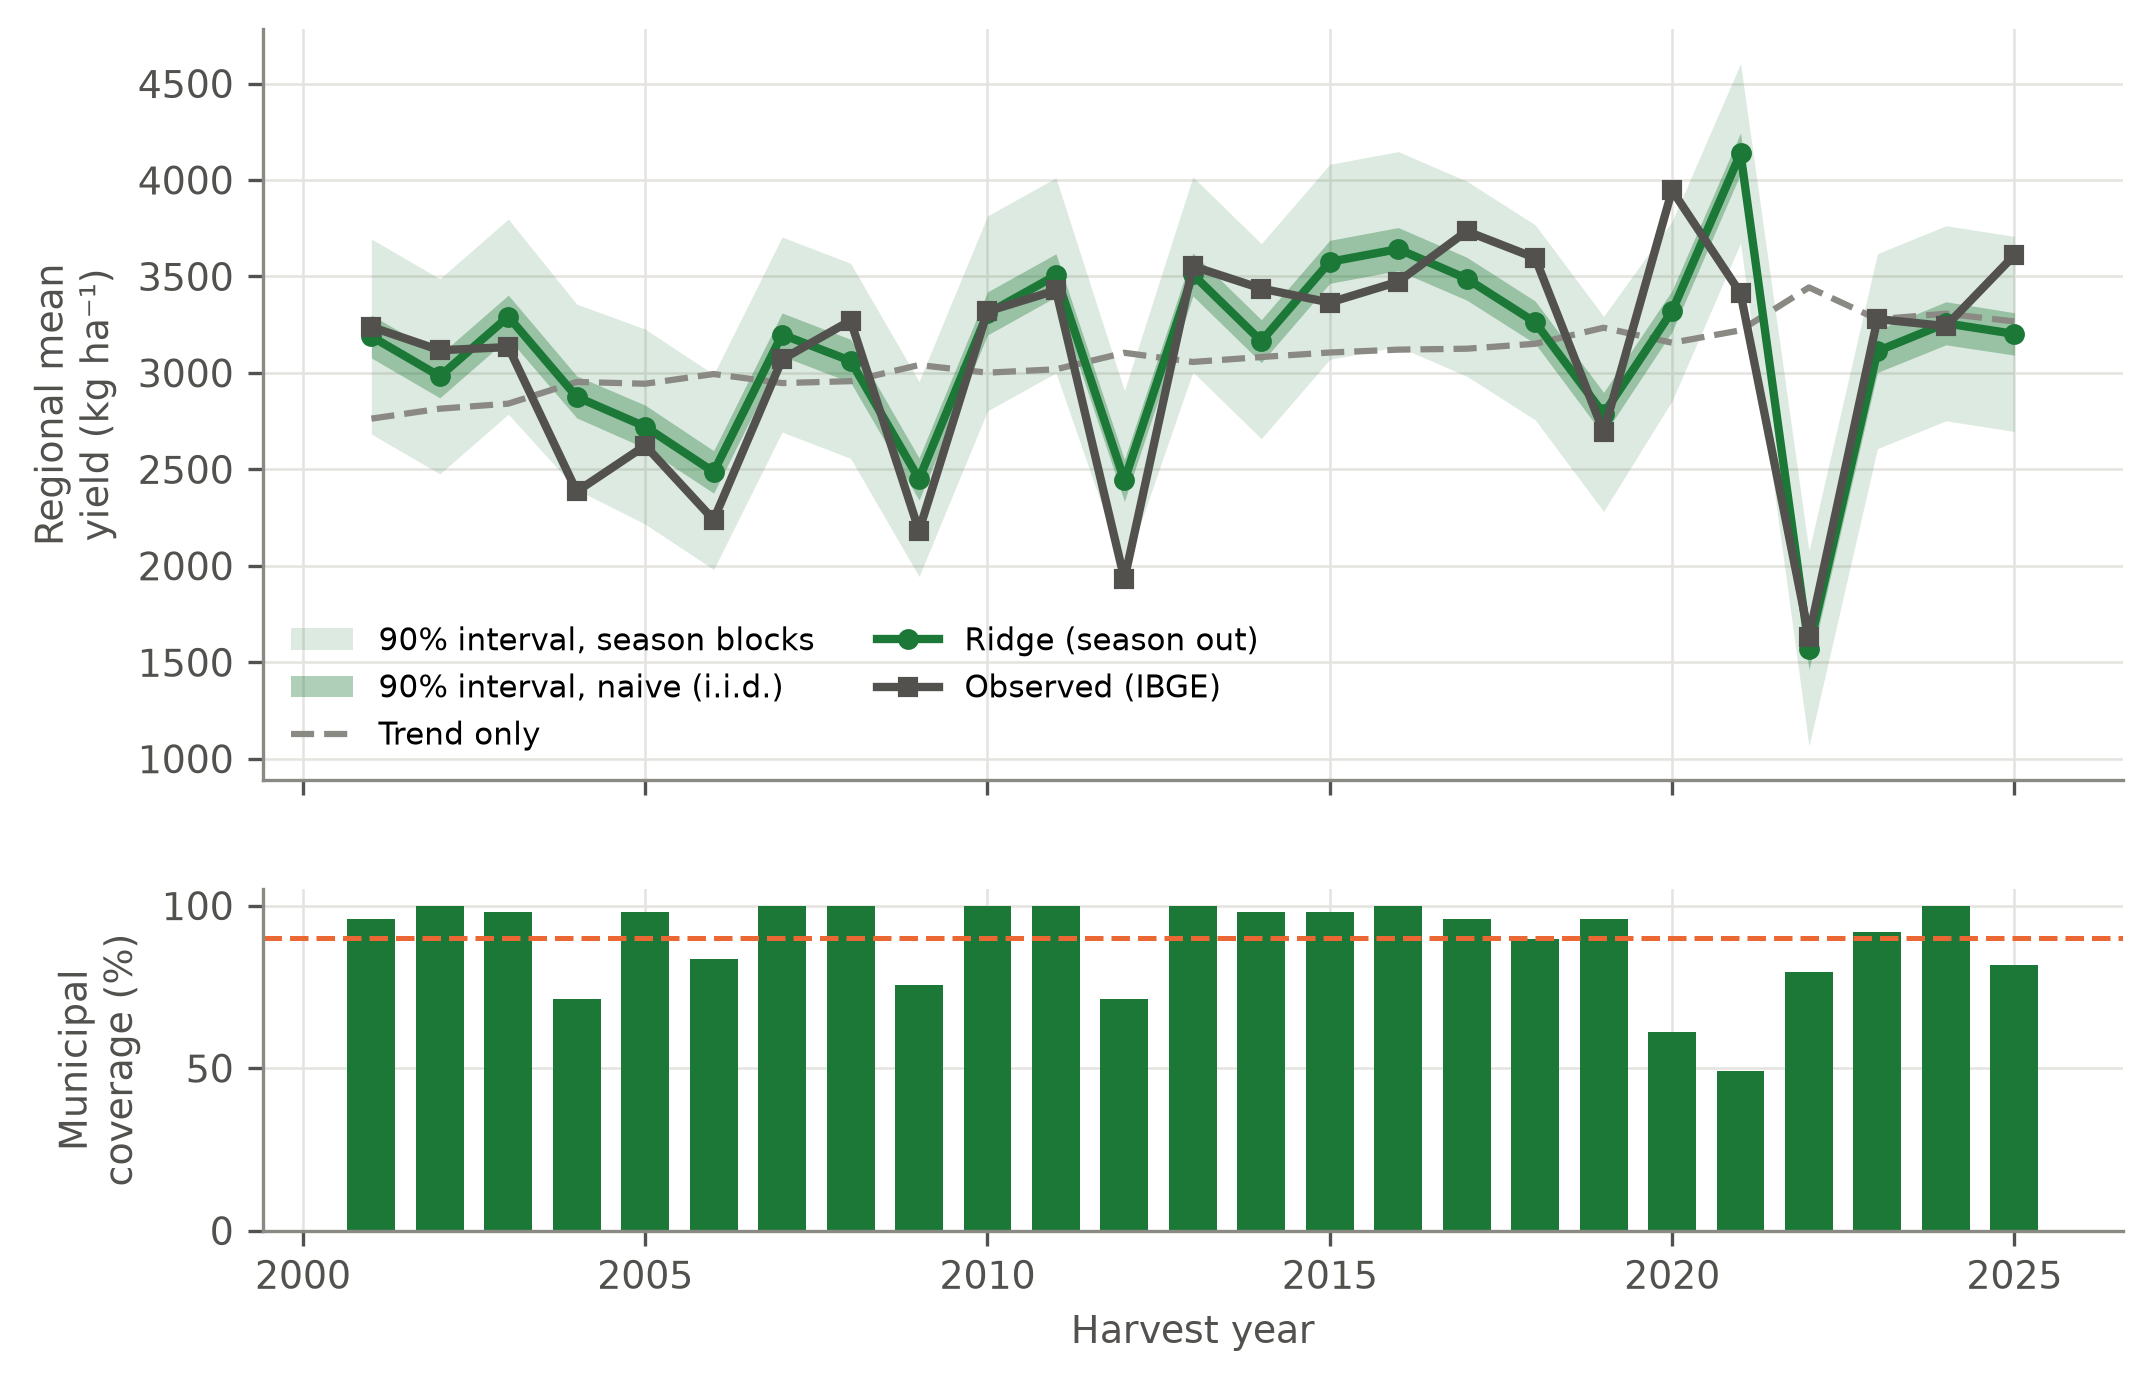
\includegraphics[width=\textwidth]{figuras/fig03_serie_regional_incerteza.png}
\caption{Regional mean yield: observed, trend and LOSO forecast of ridge regression with naive (i.i.d.) and season-block 90\% intervals (top), and coverage of the municipal split conformal 90\% intervals per season (bottom; dashed line: nominal level).}
\label{fig:ic}
\end{figure}

\begin{figure}[ht]
\centering
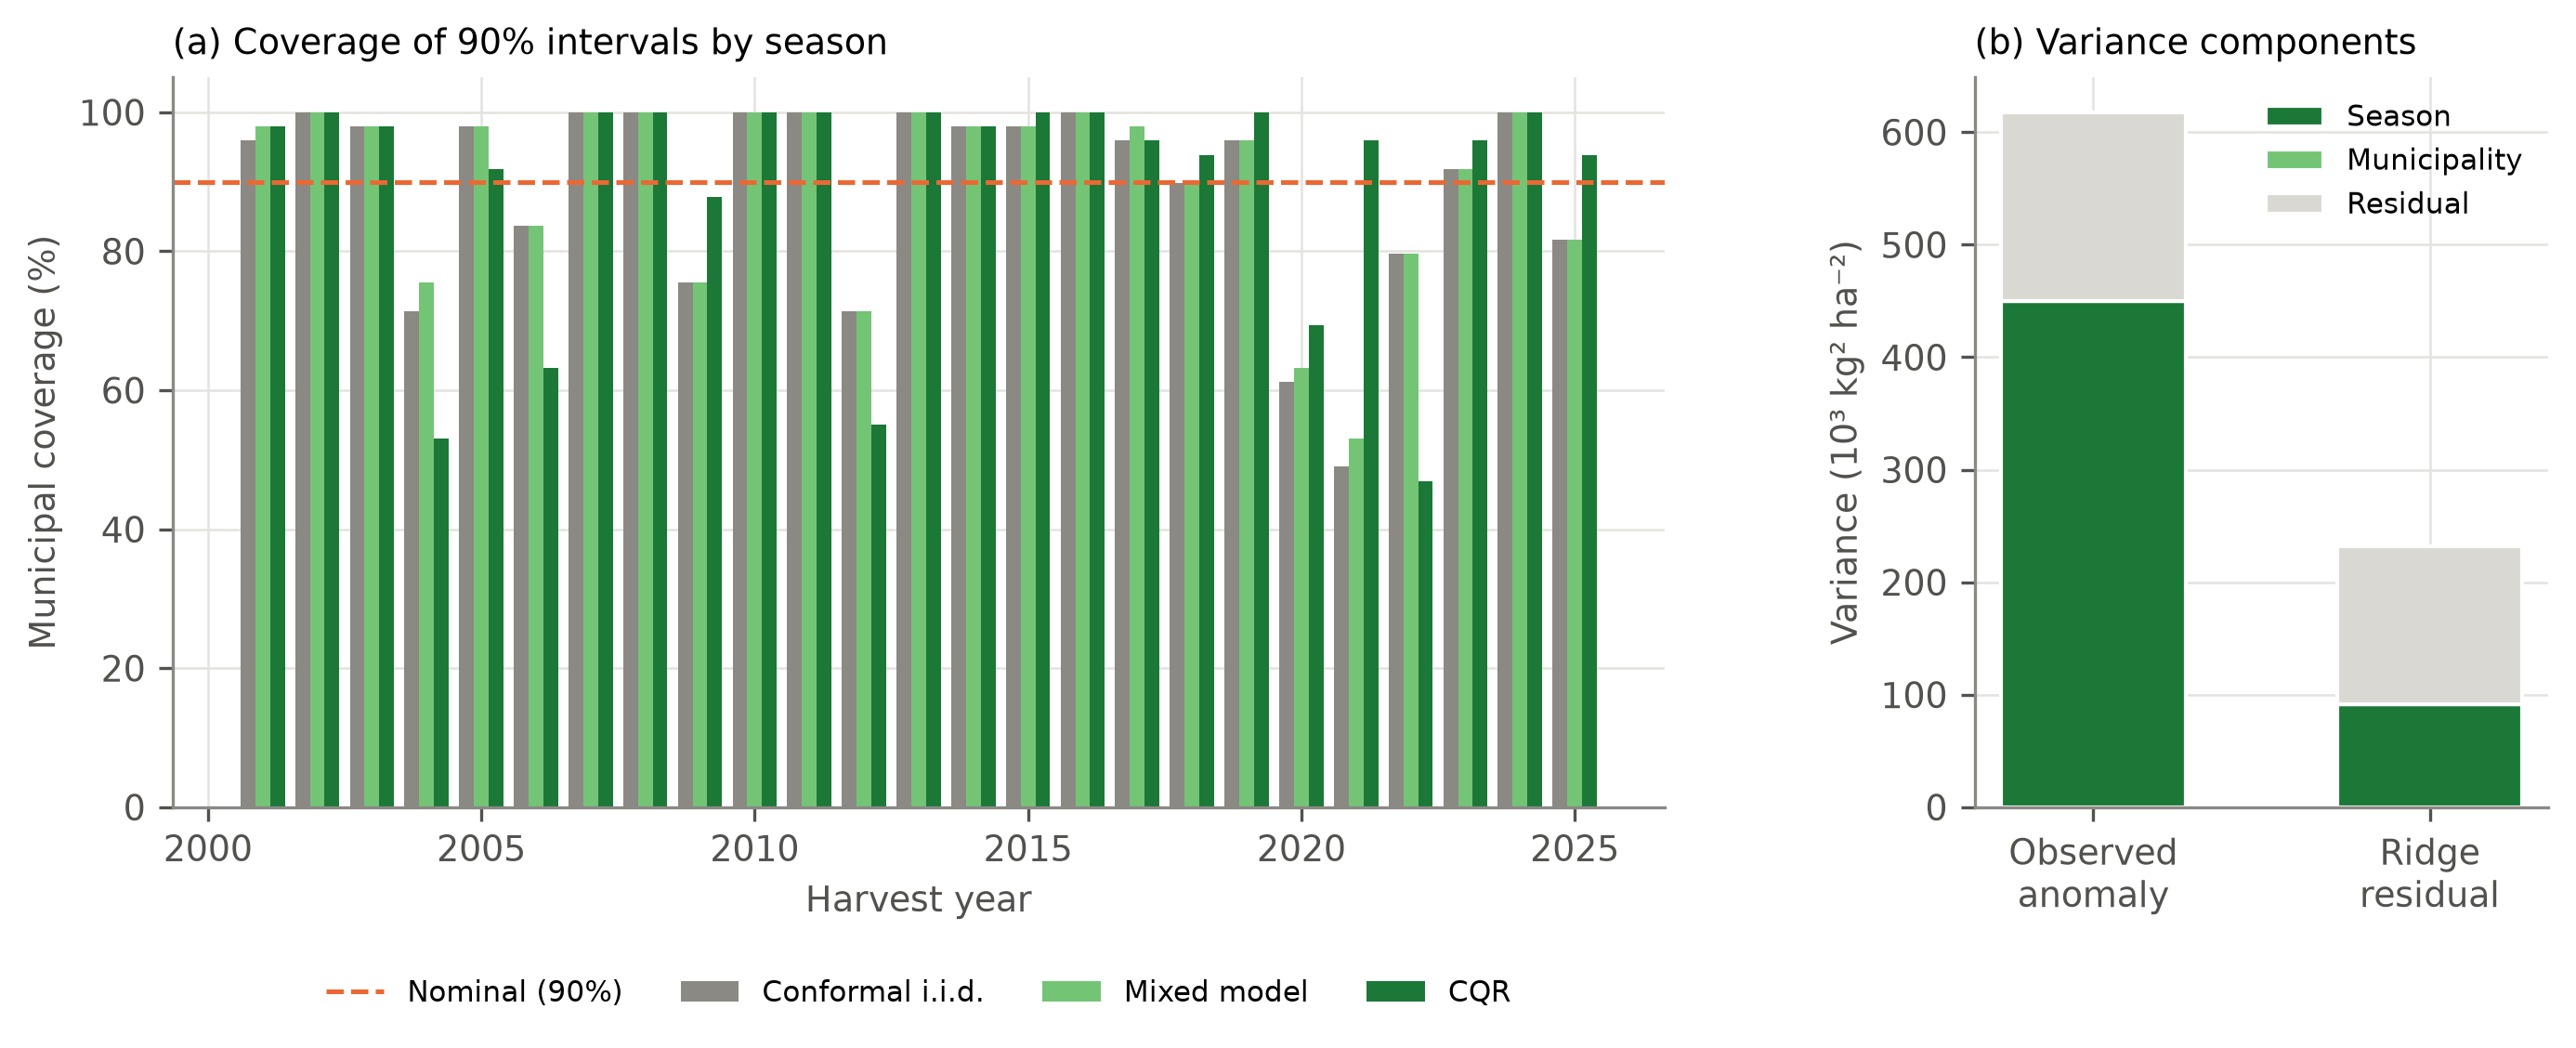
\includegraphics[width=\textwidth]{figuras/fig08_intervalos_variancia.png}
\caption{(a) Coverage of the municipal 90\% intervals by season for split conformal, mixed-model and CQR intervals; (b) variance components of the observed yield anomalies and of the LOSO residuals of ridge regression.}
\label{fig:ic8}
\end{figure}

These results follow from the error structure. Conformal intervals guarantee the nominal coverage on average over exchangeable observations \citep{lei2018,romano2019}, and this guarantee held on average over seasons, but the errors of the 49 municipalities of a season share the season component, so that in a season with a large common error most intervals fail together \citep{barber2023}. For aggregate quantities, the effective sample size is the number of seasons and not the number of records, and intervals for the regional mean that divide the municipal error by $\sqrt{n}$ are about 4.5 times too narrow. Intervals calibrated on season blocks, or derived from a model with a season random effect, recovered a coverage close to the nominal level, at the cost of widths that correctly represent the uncertainty of forecasting a new season. Spatial conformal methods \citep{mao2024}, hierarchical models with spatially correlated errors \citep{lindgren2011} and distributional regression models of yield risk \citep{pala2026} are natural extensions of this approach.

\subsection{Shortfall risk, lead time and predictor contributions}\label{sec:res_risk}
Shortfalls below 80\% of the trend occurred in 16.4\% of the municipality--seasons, and their forecast probability had a Brier score of 0.070, against 0.144 for the climatological frequency (BSS = 0.51), and an AUC of 0.94 (Fig.~\ref{fig:risco}). The skill was similar for thresholds of 70\% (frequency of 11.7\%, BSS = 0.46, AUC = 0.96) and 90\% (24.3\%, BSS = 0.52, AUC = 0.92). The reliability diagrams followed the diagonal at low and intermediate probabilities, but the observed frequency for forecast probabilities above 0.8 was about 0.8, which indicates slight overconfidence in the seasons forecast as severe.

\begin{figure}[ht]
\centering
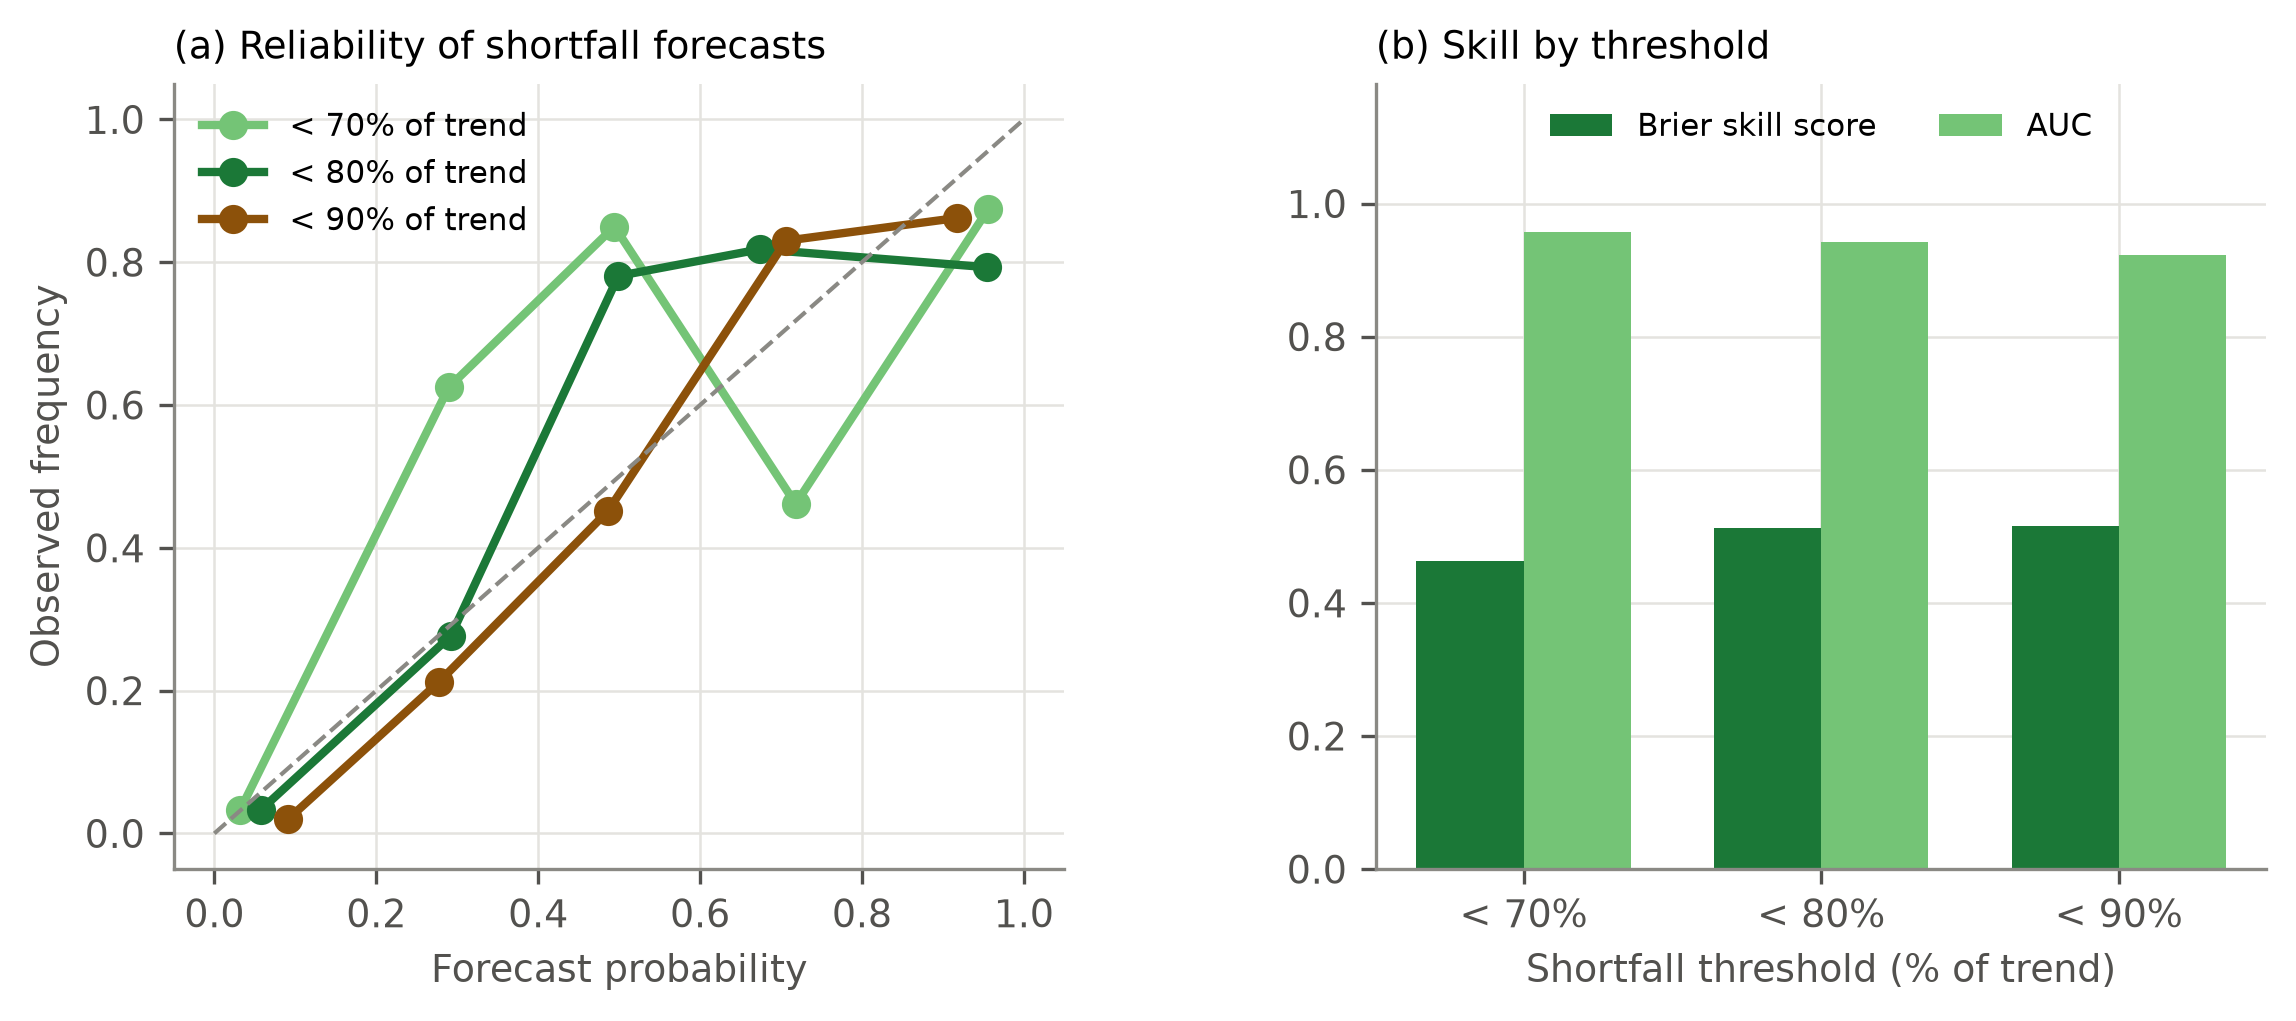
\includegraphics[width=\textwidth]{figuras/fig09_risco.png}
\caption{(a) Reliability of the forecast probability of yield shortfall below 70, 80 and 90\% of the trend; (b) Brier skill score over climatology and AUC by threshold.}
\label{fig:risco}
\end{figure}

Forecasts issued with the predictors of October had no skill (skill of $-0.02$), but the skill increased to 0.41 with the predictors up to December, to 0.54 up to January and to 0.58 at harvest (Fig.~\ref{fig:lead}). A forecast issued in early February therefore retains 93\% of the final skill, two months before the end of harvest and before the publication of the municipal statistics. \citet{Schwalbert2020} also found that the error of soybean forecasts in southern Brazil decreases from January to March, and \citet{vonBloh2023} forecast national soybean yield with useful accuracy by the end of December.

The absence of skill in October was not overcome by the El Niño--Southern Oscillation, although southern Brazil is one of the regions of the country most affected by ENSO \citep{cavalcanti2016tempo}. The Oceanic Niño Index of August--October \citep{noaa_oni} had a correlation of only 0.12 with the regional yield anomaly (0.17 for November--January); seasons under La Niña had a mean anomaly of $-2.9$\%, against $+4.5$\% under El Niño and $-1.2$\% in neutral seasons, but only two of the six seasons with losses above 15\% (2012 and 2022) occurred under La Niña, whereas 2004, 2006 and 2009 occurred in neutral conditions. Adding the index to the predictors of October did not change the skill ($-0.015$ against $-0.024$), nor did it improve the forecast at harvest (0.580 against 0.583). The losses of western Paraná therefore depend on dry spells within the season, which are not determined by the ENSO phase, and the index used by \citet{vonBloh2023} at the national scale does not replace in-season observations at the municipal scale.

\begin{figure}[ht]
\centering
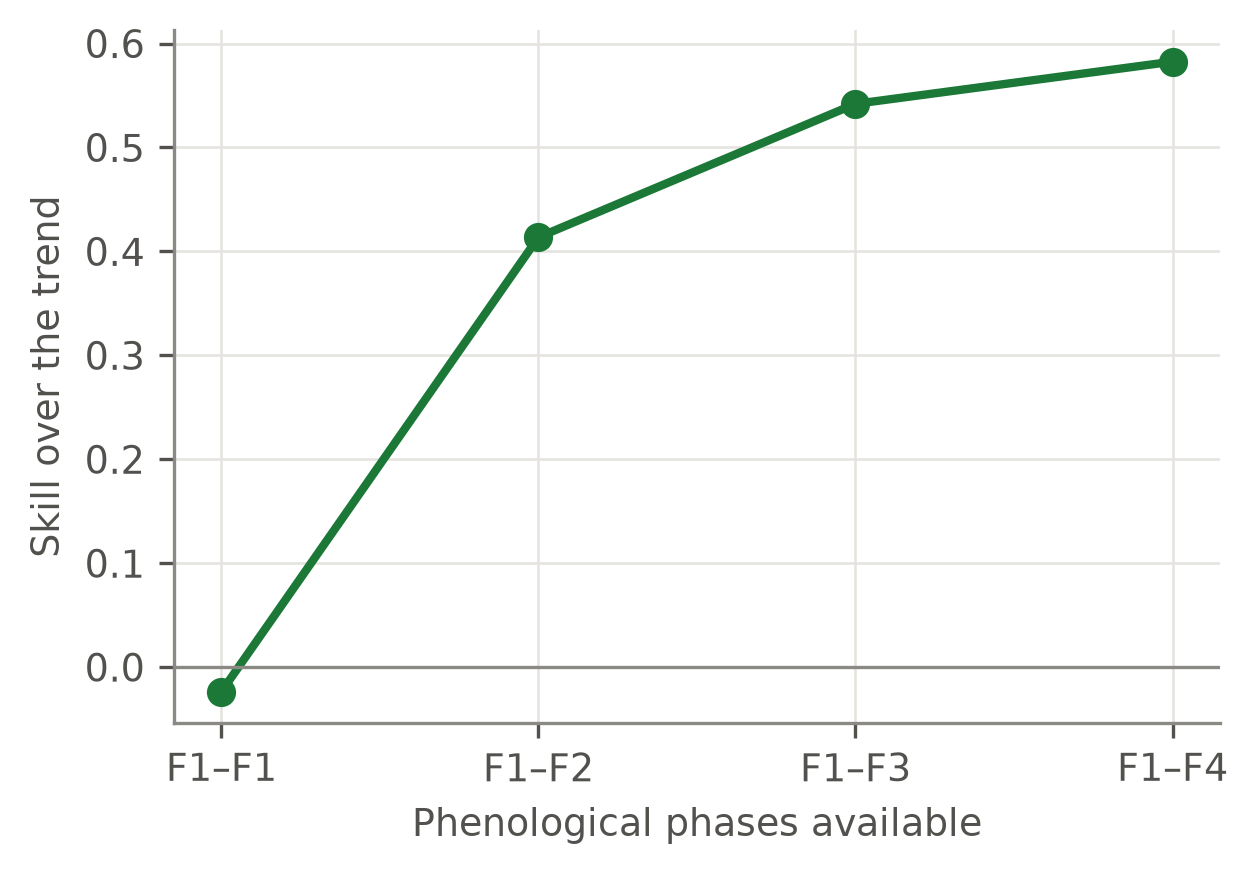
\includegraphics[width=0.6\textwidth]{figuras/fig06_antecedencia.png}
\caption{Skill of ridge regression over the trend as a function of the phenological phases available at forecast time (LOSO).}
\label{fig:lead}
\end{figure}

The contributions of the predictors were highest for phase F3 (January), followed by F1, F2 and F4, and the static predictors contributed least (Fig.~\ref{fig:shap}). The mean and maximum NDVI and EVI of January and the mean EVI and NDVI of November--December were the most important predictors, followed by the number of hot days and the absolute maximum temperature of October and by the dew-point temperature of January. Vegetation indices integrate the effect of water deficit and heat on the canopy during flowering and pod setting, the stages in which water deficit most reduces soybean yield \citep{doss1974,neumaier2000estagios,tejo2019soja}, which explains their dominance over the weather variables; NDVI and EVI respond to leaf area and canopy vigour \citep{huang2021commentary,formaggio2017sensoriamento}, so that a crop stressed in December or January shows lower indices before the loss of yield is realised. The contribution of October temperatures should be interpreted with caution: hot and dry springs preceded several of the drought seasons, so that this predictor may act as an early indicator of the seasonal regime rather than as a direct cause of yield losses.

\begin{figure}[ht]
\centering
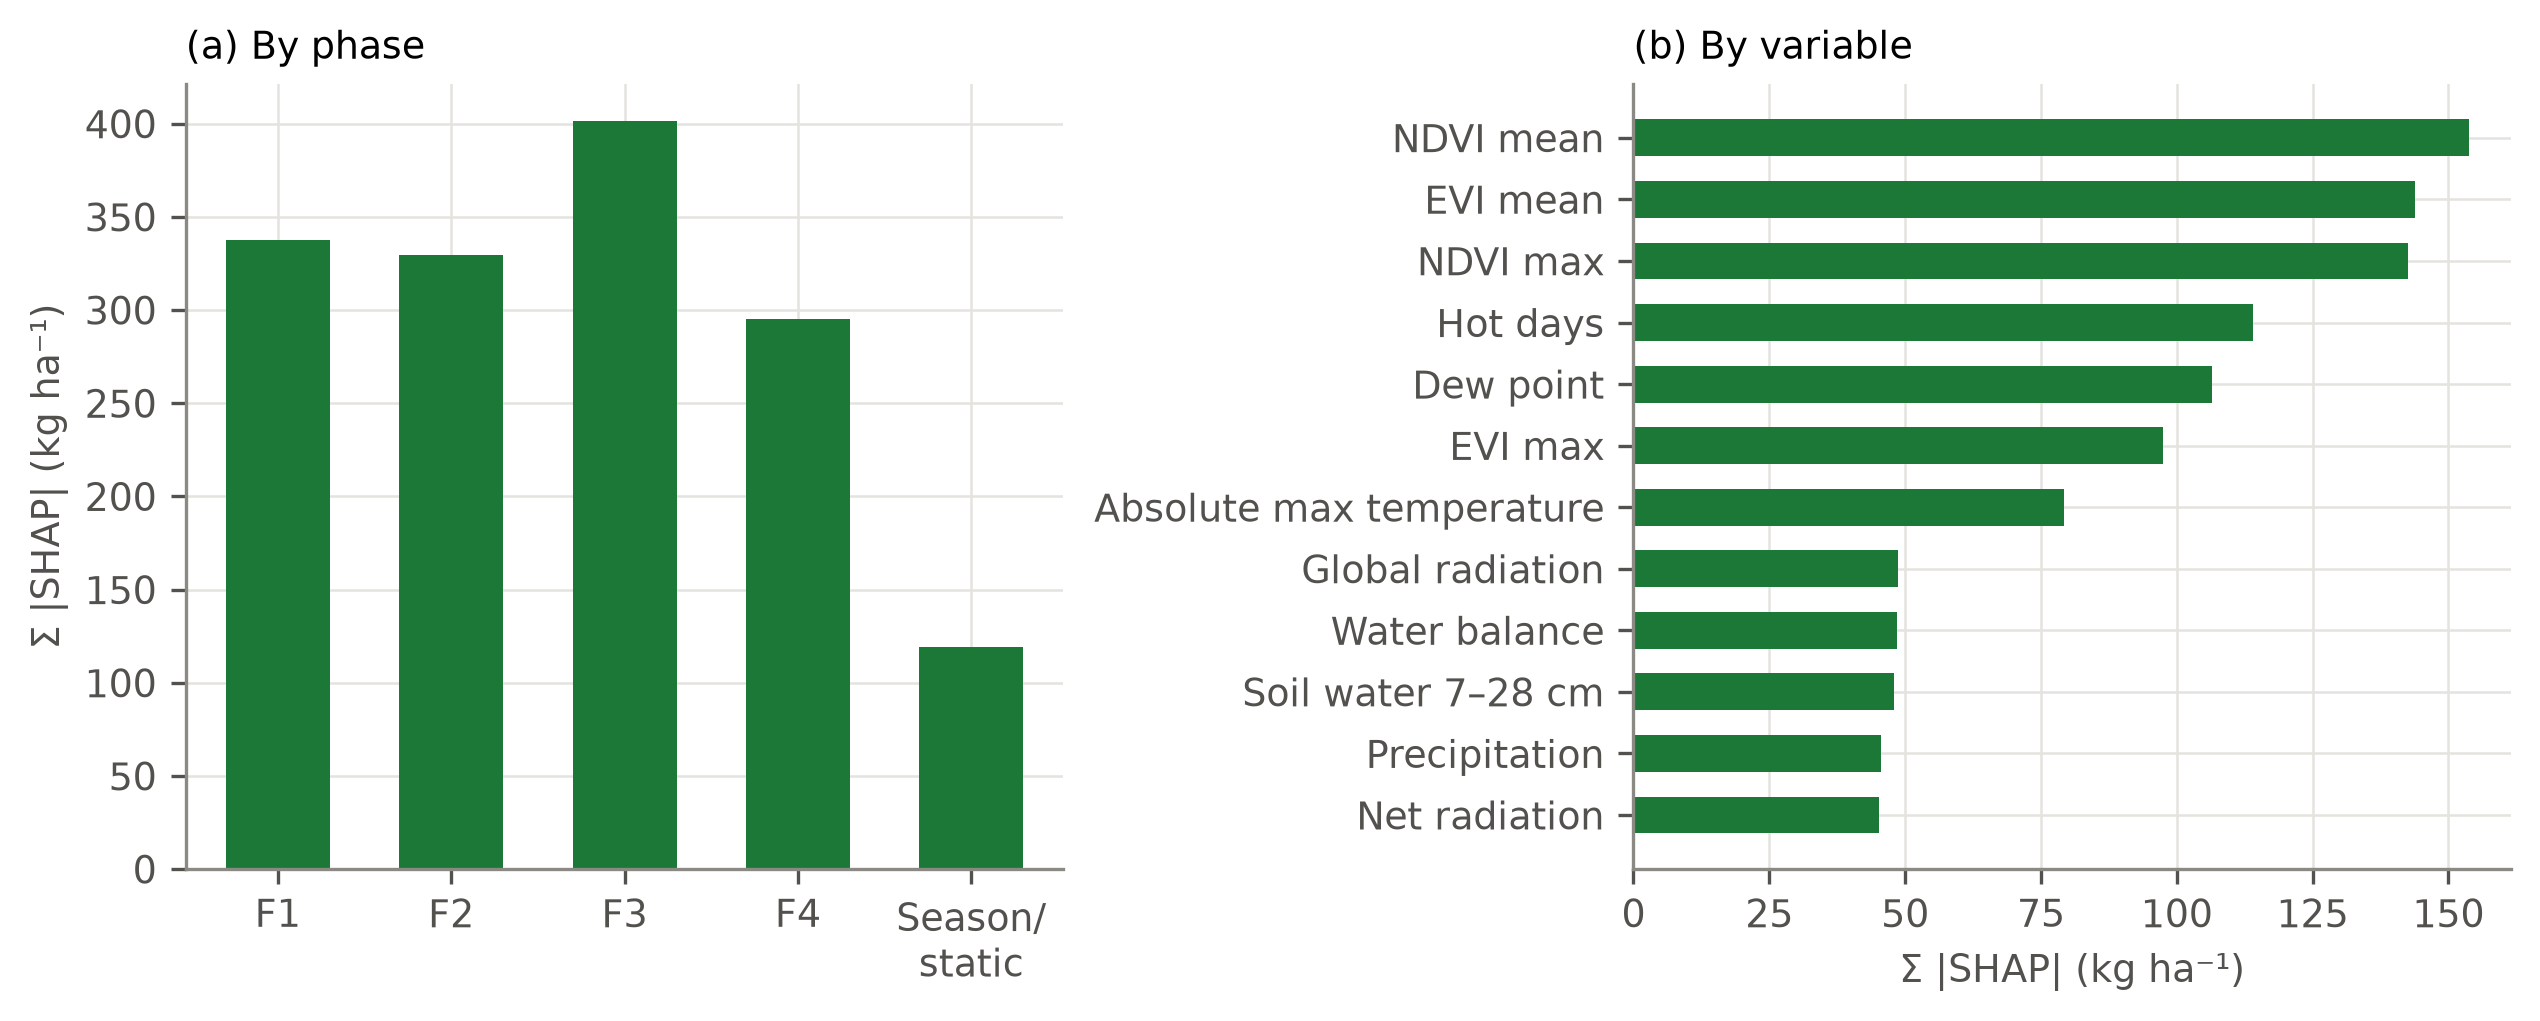
\includegraphics[width=\textwidth]{figuras/fig07_shap.png}
\caption{Mean absolute SHAP contribution of the predictors of ridge regression (a) by phase and (b) by variable.}
\label{fig:shap}
\end{figure}

\subsection{Systemic risk and implications for crop insurance}\label{sec:res_seguro}
The season component of the yield anomalies is, from the point of view of an insurer, a systemic risk: in 2022, 38 of the 49 municipalities had yields below 80\% of the trend, and in 2012, 39, so that losses that could be diversified across municipalities in a normal season occurred together. The drought of 2021/22 caused losses estimated at R\$ 22.5 billion for soybean and maize in Paraná \citep{gazetadopovo2022seca}. Spatially correlated losses are the main reason why crop insurance markets depend on reinsurance and public support \citep{miranda1997}, and weather risk in agriculture has a systemic component that limits the diversification of losses in space \citep{xu2010}, consistent with the dependence over the whole region found here (Section~\ref{sec:res_err}).

Three implications follow for the use of yield forecasts in insurance and planning. First, the regional loss forecast in early February, with its season-block interval, is the relevant quantity for an insurer or a cooperative, and the naive interval, 4.5 times narrower, would underestimate the reserves needed in a drought season. Second, the probability of shortfall by municipality (AUC = 0.94) can complement the agricultural climate risk zoning \citep{brasil2025zarc}, which defines the sowing windows eligible for insurance but does not forecast the current season. Third, because the distribution of yields, and not only its mean, determines the premium and the indemnities, distributional models of yield risk \citep{pala2026} should be evaluated with the same season-blocked design used here, otherwise the dependence between municipalities will also make their risk estimates overconfident.

\subsection{Limitations}\label{sec:lim}
The phases were defined by calendar dekads, whereas the development of soybean depends on the sowing date, the cultivar and the response to temperature and photoperiod \citep{CONSTABLE198857}; in seasons with late sowing, part of the flowering falls in phase F3 instead of F2, which blurs the association between phases and stages. Reanalysis variables have their own uncertainties, which are larger where observations are scarce \citep{GUALTIERI2022112741,munozsabater2021}. The study is also limited by the 25 seasons available, which constrain both model complexity and the calibration of intervals for extreme seasons, and by the municipal yield statistics, which are estimates subject to revision and do not separate first- and second-crop soybean or irrigated areas \citep{sidra}. MODIS pixels at 250 m mix soybean with other land uses at the edges of fields, and the MapBiomas soybean class has its own classification errors \citep{souza2020}. The analysis was restricted to western Paraná; regions with less spatially coherent weather, or with a larger number of municipalities and seasons, may show a smaller season component and a smaller cost of ignoring it.

%% ---------------------------------------------------------------
\section{Conclusions}\label{sec:conc}
\begin{itemize}
\item Random and leave-one-municipality-out validation of municipal soybean yield forecasts in western Paraná gave $R^2$ of about 0.80 even with yields paired to the weather of the wrong season; only validation that leaves out whole seasons measured forecast skill.
\item Under season-blocked validation, ridge regression on phase-aggregated MODIS indices and ERA5-Land and CHIRPS variables reduced the mean squared error of the technological trend by 58\% ($R^2 = 0.59$), outperforming tree-based models, and a forecast in early February retained 93\% of this skill; Landsat did not add information to MODIS.
\item The season effect common to all municipalities accounted for 73\% of the variance of yield anomalies and 40\% of the forecast residuals, and residuals were spatially autocorrelated in 22 of 25 seasons; prediction intervals that ignored this dependence covered the regional mean yield in 32\% of the seasons, against 84\% for season-block and mixed-model intervals.
\item The probability of a yield shortfall below 80\% of the trend was forecast with a Brier skill score of 0.51 over climatology and an AUC of 0.94, which supports the use of season-validated forecasts with calibrated uncertainty for crop insurance and planning in the region.
\end{itemize}

\backmatter

\bmhead{Supplementary information}
The Supplementary Material contains the list of predictors, the results of all datasets, validation schemes and models, the bootstrap comparisons and trend forms, the performance by municipality, the results by season (regional yield, Moran's $I$ and interval coverage), the skill and reliability of shortfall forecasts, and the semivariogram of the residuals.

\bmhead{Acknowledgements}
\inserir{agradecimentos e bolsas}.

\section*{Declarations}
\begin{itemize}
\item \textbf{Funding} \inserir{}
\item \textbf{Competing interests} The authors declare no competing interests.
\item \textbf{Data availability} Municipal predictors by season, LOSO forecasts and all evaluation results are available at \inserir{repositório GitHub/Zenodo}. Yield data are public (IBGE, table 1612).
\item \textbf{Code availability} \inserir{GitHub}.
\item \textbf{Author contributions} \inserir{}
\end{itemize}

\bibliography{referencias}

\end{document}
